





\documentclass{beamer}
%  \usepackage[utf8]{inputenc}
\usepackage[utf8]{inputenc}
  \usetheme{Warsaw}
  \usepackage{dsfont}
  \usepackage{xcolor}
%  \usepackage[dvipsnames]{xcolor}
  \usepackage{tabto}

\usepackage{mathtools}
\usepackage{todonotes}
\usepackage{microtype}

\usepackage{complexity}
\usepackage{amsmath}

\usepackage{stmaryrd}
\usepackage{dsfont}

 \usepackage{cancel}

\usepackage{mathrsfs}
\usepackage{mathalpha}
\usepackage{amsmath}
\usepackage{amsfonts}
\usepackage{multirow}

\usepackage{ textcomp } 

\usepackage{stmaryrd}
\usepackage{wrapfig}


\title[Resilience and Home-Space for WSTS]{Resilience and Home-Space for WSTS}

\author[Alain Finkel ~ Mathieu Hilaire]{Alain Finkel \inst{1} \and Mathieu Hilaire \inst{2}}
\institute[Alain Finkel ~ Mathieu Hilaire]{\inst{1} Université Paris-Saclay, CNRS, ENS Paris-Saclay, LMF, Gif-sur-Yvette, France, Institut Universitaire de France \and %
                      \inst{2} Université Lyon 1, LIRIS, France}

\date{}

\setbeamertemplate{page number in head/foot}[totalframenumber]



\usepackage{pgf}
\usepackage{tikz}
\usetikzlibrary{arrows,automata}
%\usepackage[latin1]{inputenc}

\bibliographystyle{alpha}% the recommnded bibstyle

\newcommand{\Z}{\mathbb{Z}}
\newcommand{\N}{\mathbb{N}}


\colorlet{Mycolor1}{green!10!orange!90!}
\colorlet{Mycolor3}{blue!20!magenta!90!}
\definecolor{Mycolor2}{HTML}{00F9DE}


\newcommand{\pred}{\textsf{pred}}
\newcommand{\post}{\textsf{post}}



\newcommand{\Bad}{\textsf{Bad}}
\newcommand{\Safe}{\textsf{Safe}}


\begin{document}


\maketitle


%vvvvvvvvvvvvvvvvvvvvvvvvvvvvvvvvvvvvvvvvvvvvvvvvvvvvvvvvvvvvvvvvvvvvvvvvvv
%  \begin{frame}{Outline}

%\tableofcontents
%  \end{frame}
  \section{Introduction}
%vvvvvvvvvvvvvvvvvvvvvvvvvvvvvvvvvvvvvvvvvvvvvvvvvvvvvvvvvvvvvvvvvvvvvvvvvv
  \begin{frame}{Motivation}

\begin{columns}[T]
 \column{0.35\textwidth}
 \begin{figure}
 	\hspace{-0.5cm}

\includegraphics[width=1.\textwidth]{fridge}
% \caption{Hasse diagram of some classes of transition systems, together with the decidability (in green) or undecidability (in red) of the resilience problems. Decidability of bounded resilience and $k-$resilience variants are indicated in blue.}
\end{figure} 

 \column{0.65\textwidth}
\phantom{Fridge.png} \\
\phantom{Fridge.png} \\
{\sf Bad} state = temperature $\geq 6^\circ C$ \newline

 {\sf Good} state = temperature $\leq 6^\circ C$ \\

\end{columns}

\pause

\phantom{Fridge.png} \\
Other applications e.g.  nuclear reactor 

\iffalse
  \todo[inline,color=blue!20]{ {\it À l'oral~}
We are usually focused on how to avoid bad states in general but you can see when your fridge the system stops providing refrigerating temperature it's not over yet
If you leave your fridge off for a minute it's not going to have Terrible impact but if you leave it off for more than one hour you're gonna have to throw the things in it away

And I've been talking like your frige at home but it apply to any type of cooling system it can be like refrigerating medical supplies or nuclear reactor.

And this is interesting Bcz now the stuff is not necessarily avoid bad states completely

This lead to concept of resilience
}
\fi

  \end{frame}
%vvvvvvvvvvvvvvvvvvvvvvvvvvvvvvvvvvvvvvvvvvvvvvvvvvvvvvvvvvvvvvvvvvvvvvvvvv
  \begin{frame}{Example: Reset-VASS $V_1$}
  
  
   \begin{center}
 	\begin{figure}
 	\vspace{.06cm}
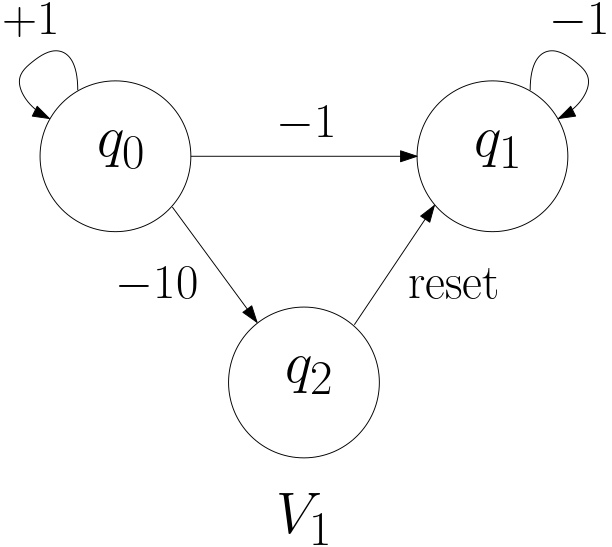
\includegraphics[width=.4\textwidth]{FigA}
	\end{figure}
\end{center}  


\begin{columns}[T]
 \column{0.6\textwidth}

$\Safe_1 = \{q_0(n) \mid n \in \N\}$

\vspace{0.1cm}

$\Safe_2 = \{q_1(0)\} $




 \column{0.4\textwidth}
 
\phantom{ {resilience} }

\vspace{0.1cm}

\phantom{ {resilience} }

\end{columns}


  \end{frame}
%vvvvvvvvvvvvvvvvvvvvvvvvvvvvvvvvvvvvvvvvvvvvvvvvvvvvvvvvvvvvvvvvvvvvvvvvvv
  \begin{frame}{Resilience problems}
  

% TODO

% Define the Six different problems we study/focus on.

% (Takes some room but I think mb having the six on the same page could be better than having three then three state-* on two separate pages ?)
  

\hspace{-0.5cm}  {\bf INPUT:\ }{A transition system $\mathscr{S}=(S,\rightarrow)$, and a set $\Safe \subseteq S$, \\ $\Bad$ complement of $\Safe$.}

\hspace{-0.5cm}  {\bf QUESTION:\ } 

\begin{columns}[T]
 \column{0.3\textwidth}

  $\Bad \rightarrow^{*} \Safe$  ?

\vspace{0.15cm}

   $\Bad \rightarrow^{\leq k} \Safe$  ?

\vspace{0.15cm}

  $\exists k ~ \Bad \rightarrow^{\leq k} \Safe$   ?\newline

 \column{0.7\textwidth}
 
\hspace{0.6cm} {\sc  \phantom{bounded} resilience problem}

\vspace{0.16cm}

\hspace{0.6cm} {\sc \phantom{boundi} $k$-resilience problem}

\vspace{0.175cm}

\hspace{0.6cm} {\sc bounded resilience problem}

\end{columns}

  \end{frame}
%vvvvvvvvvvvvvvvvvvvvvvvvvvvvvvvvvvvvvvvvvvvvvvvvvvvvvvvvvvvvvvvvvvvvvvvvvv
  \begin{frame}{Example: Reset-VASS $V_1$}
  
  
   \begin{center}
 	\begin{figure}
 	\vspace{.06cm}
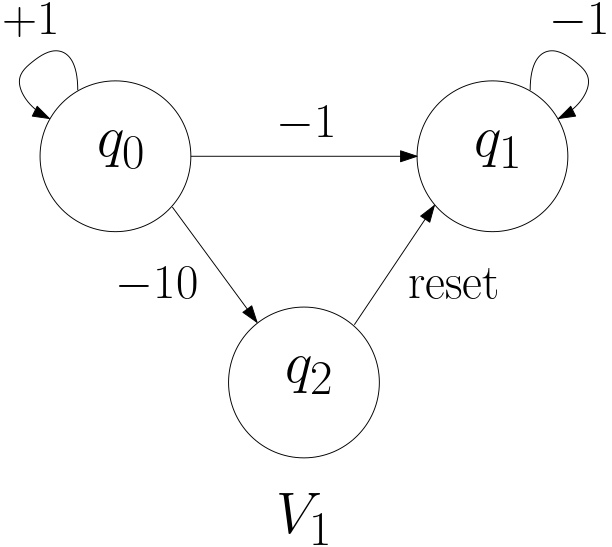
\includegraphics[width=.4\textwidth]{FigA}
	\end{figure}
\end{center}  

\only<1>{
\begin{columns}[T]
 \column{0.6\textwidth}

$\Safe_1 = \{q_0(n) \mid n \in \N\}$ 	

 \column{0.4\textwidth}
 
 Resilience(s) not satisfied

\vspace{0.1cm}

\phantom{bla} $q_1(m) ~ \cancel{\to} ~ q_0(n)$

\end{columns}

}


\only<2>{
\begin{columns}[T]
 \column{0.6\textwidth}

$\Safe_2 = \{q_1(0)\} $

 \column{0.4\textwidth}
 
 Resilience hold, 
 
 \vspace{0.1cm}
 
 \hspace{-0.6cm} Bounded resilience does not

\end{columns}

}


  \end{frame}
%vvvvvvvvvvvvvvvvvvvvvvvvvvvvvvvvvvvvvvvvvvvvvvvvvvvvvvvvvvvvvvvvvvvvvvvvvv
  \begin{frame}{Example: Reset-VASS $V_2$}
  
  
   \begin{center}
 	\begin{figure}
% 	\hspace{-2.cm}
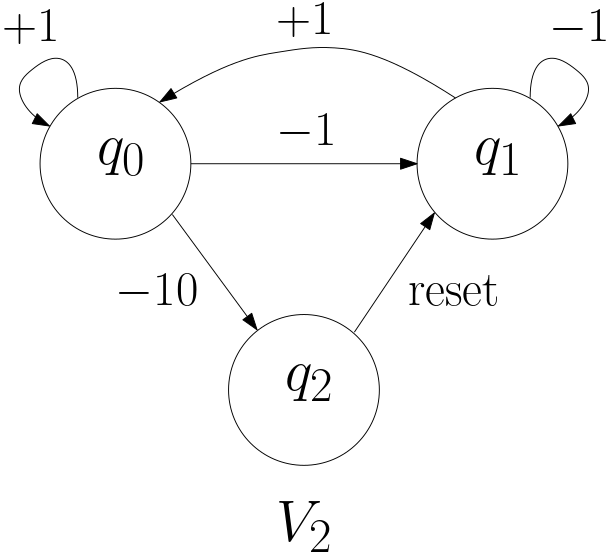
\includegraphics[width=.4\textwidth]{FigB}
	\end{figure}
\end{center}  

\begin{columns}[T]
 \column{0.6\textwidth}

$\Safe_2 = \{q_1(0)\} $

 \column{0.4\textwidth}
 
 Bounded resilience hold, 
 
 \vspace{0.1cm}
 
 \phantom{bla} $6$-resilience hold

\end{columns}

 \vspace{0.1cm}
 
$q_1(7) \to q_0(8) \to q_0(9) \to q_0(10) \to q_2(0) \to q_1(0)$

$q_1(6) \to q_1(5) \to q_1(4) \to q_1(3) \to q_1(2) \to q_1(1) \to q_1(0)$

  \end{frame}
%vvvvvvvvvvvvvvvvvvvvvvvvvvvvvvvvvvvvvvvvvvvvvvvvvvvvvvvvvvvvvvvvvvvvvvvvvv
  \begin{frame}{{State} resilience problems}
  

% TODO

% Define the Six different problems we study/focus on.

% (Takes some room but I think mb having the six on the same page could be better than having three then three state-* on two separate pages ?)
  

\hspace{-0.5cm}  {\bf INPUT:\ }{A transition system $\mathscr{S}=(S,\rightarrow)$, and a set $\Safe \subseteq S$, \\ $\Bad$ complement of $\Safe$, \textcolor{red}{$s \in S$}.}

\hspace{-0.5cm}  {\bf QUESTION:\ } 

\begin{columns}[T]
 \column{0.45\textwidth}

  $\cancel{\Bad}~\textcolor{red}{\post^*(s) } \rightarrow^{*} \Safe$  ?

\vspace{0.15cm}

   $\cancel{\Bad}~\textcolor{red}{\post^*(s) } \rightarrow^{\leq k} \Safe$  ?

\vspace{0.15cm}

  $\exists k ~ \cancel{\Bad}~\textcolor{red}{\post^*(s) } \rightarrow^{\leq k} \Safe$   ?\newline

 \column{0.7\textwidth}
 
\hspace{0.6cm} {\sc  \phantom{bounded} state-resilience problem}

\vspace{0.19cm}

\hspace{0.6cm} {\sc \phantom{boundi} $k$-state-resilience problem}

\vspace{0.20cm}

\hspace{0.6cm} {\sc bounded-state-resilience problem}

\end{columns}




 

% \todo[inline,color=blue!20]{{\bf  \tiny (Takes some room but I think mb having the six on the same page could be better than having three then three state-* on two separate pages ?)}} 



  \end{frame}
%vvvvvvvvvvvvvvvvvvvvvvvvvvvvvvvvvvvvvvvvvvvvvvvvvvvvvvvvvvvvvvvvvvvvvvvvvv
	\section{WBTS, WSTS}
  \begin{frame}{}
  
  \begin{block}{Definition~\cite{DBLP:journals/lmcs/BlondinFM17}}
A {\em Well-Behaved Transition System} (WBTS) 
is an ordered transition system $\mathscr{S}=(S, \rightarrow, \leq)$ such that   
all antichains of $(S, \leq)$ are finite, and
%the transition relation 
$ \rightarrow$ is upward-compatible with $\leq$. 
%$s_1, t_1 , s_2 \in S$
%	with $s_1 \leq s_2$  and $s_1 \rightarrow t_1$, there exists 
%	$t_2 \in S$ with 
%	$t_1 \leq t_2$ and $s_2 \rightarrow^{*} t_2$.
\end{block}

   \begin{center}
 	\begin{figure}
 	% \hspace{-2.cm}
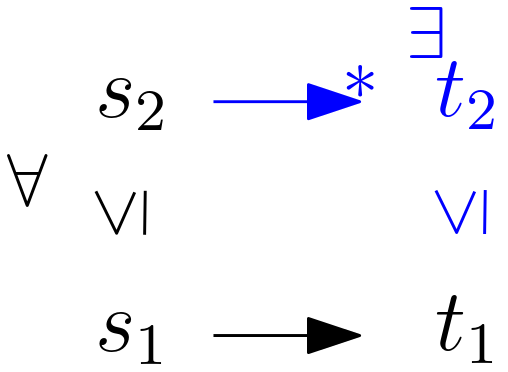
\includegraphics[width=.25\textwidth]{WSTS_def}
	\end{figure}
\end{center}  

\begin{block}{Definition~\cite{DBLP:journals/iandc/Finkel90}}
A {\em Well-Structured Transition System} (WSTS) 
is a well-ordered WBTS.
% ward) compatible with $\leq$, i.e., for all 
%$s_1, t_1 , s_2 \in S$
%	with $s_1 \leq s_2$  and $s_1 \rightarrow t_1$, there exists 
%	$t_2 \in S$ with 
%	$t_1 \leq t_2$ and $s_2 \rightarrow^{*} t_2$.
\end{block}


\pause


\begin{theorem}
{\sc Resilience} undecidable for WSTS
\end{theorem}


% \todo[inline,color=blue!20]{    \tiny
% diapo 5: théorème: c'est indécidable dans le cas général des systèmes de transitions
% diapo 5: déjà pour les bien structurés c'est indécidable
% résilience indécidable pour les post effectif WSTS quelque soit safe clos par le haut ou par le bas
% }

%  \todo[inline,color=blue!20]{    \tiny Definition right now is very formal for a slideshow, maybe make it less verbose? }





  \end{frame}
%vvvvvvvvvvvvvvvvvvvvvvvvvvvvvvvvvvvvvvvvvvvvvvvvvvvvvvvvvvvvvvvvvvvvvvvvvv
  \begin{frame}{WBTS Taxonomy}
  
   \begin{center}
 	\begin{figure}
% 	\hspace{-2.cm}
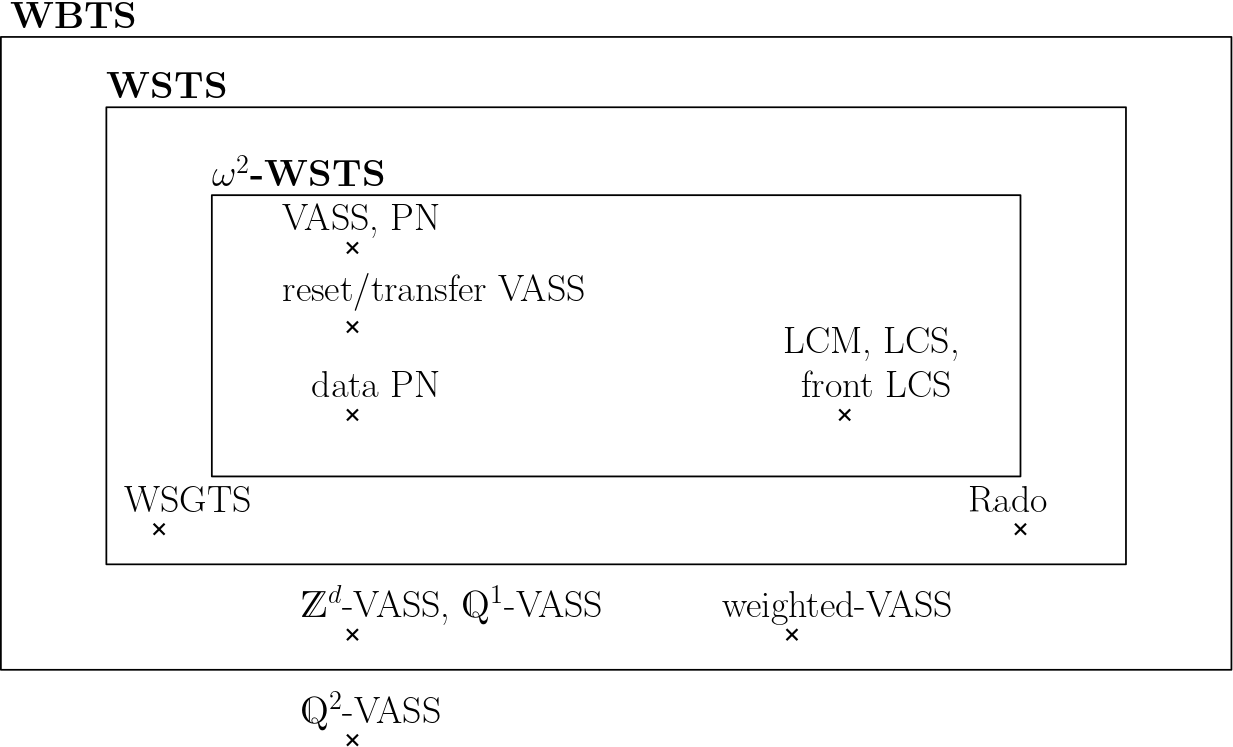
\includegraphics[width=.80\textwidth]{WSTS_taxonomy_large}
	\end{figure}
\end{center}  




  \end{frame}
%vvvvvvvvvvvvvvvvvvvvvvvvvvvvvvvvvvvvvvvvvvvvvvvvvvvvvvvvvvvvvvvvvvvvvvvvvv
	\section{Resiliences}
  \begin{frame}{Results}
  
% Now that everything is somewhat properly defined maybe the picture with all the results ?  
  
   \begin{center}
 	\begin{figure}
 	% \hspace{-2.cm}
 	\vspace{-0.25cm}
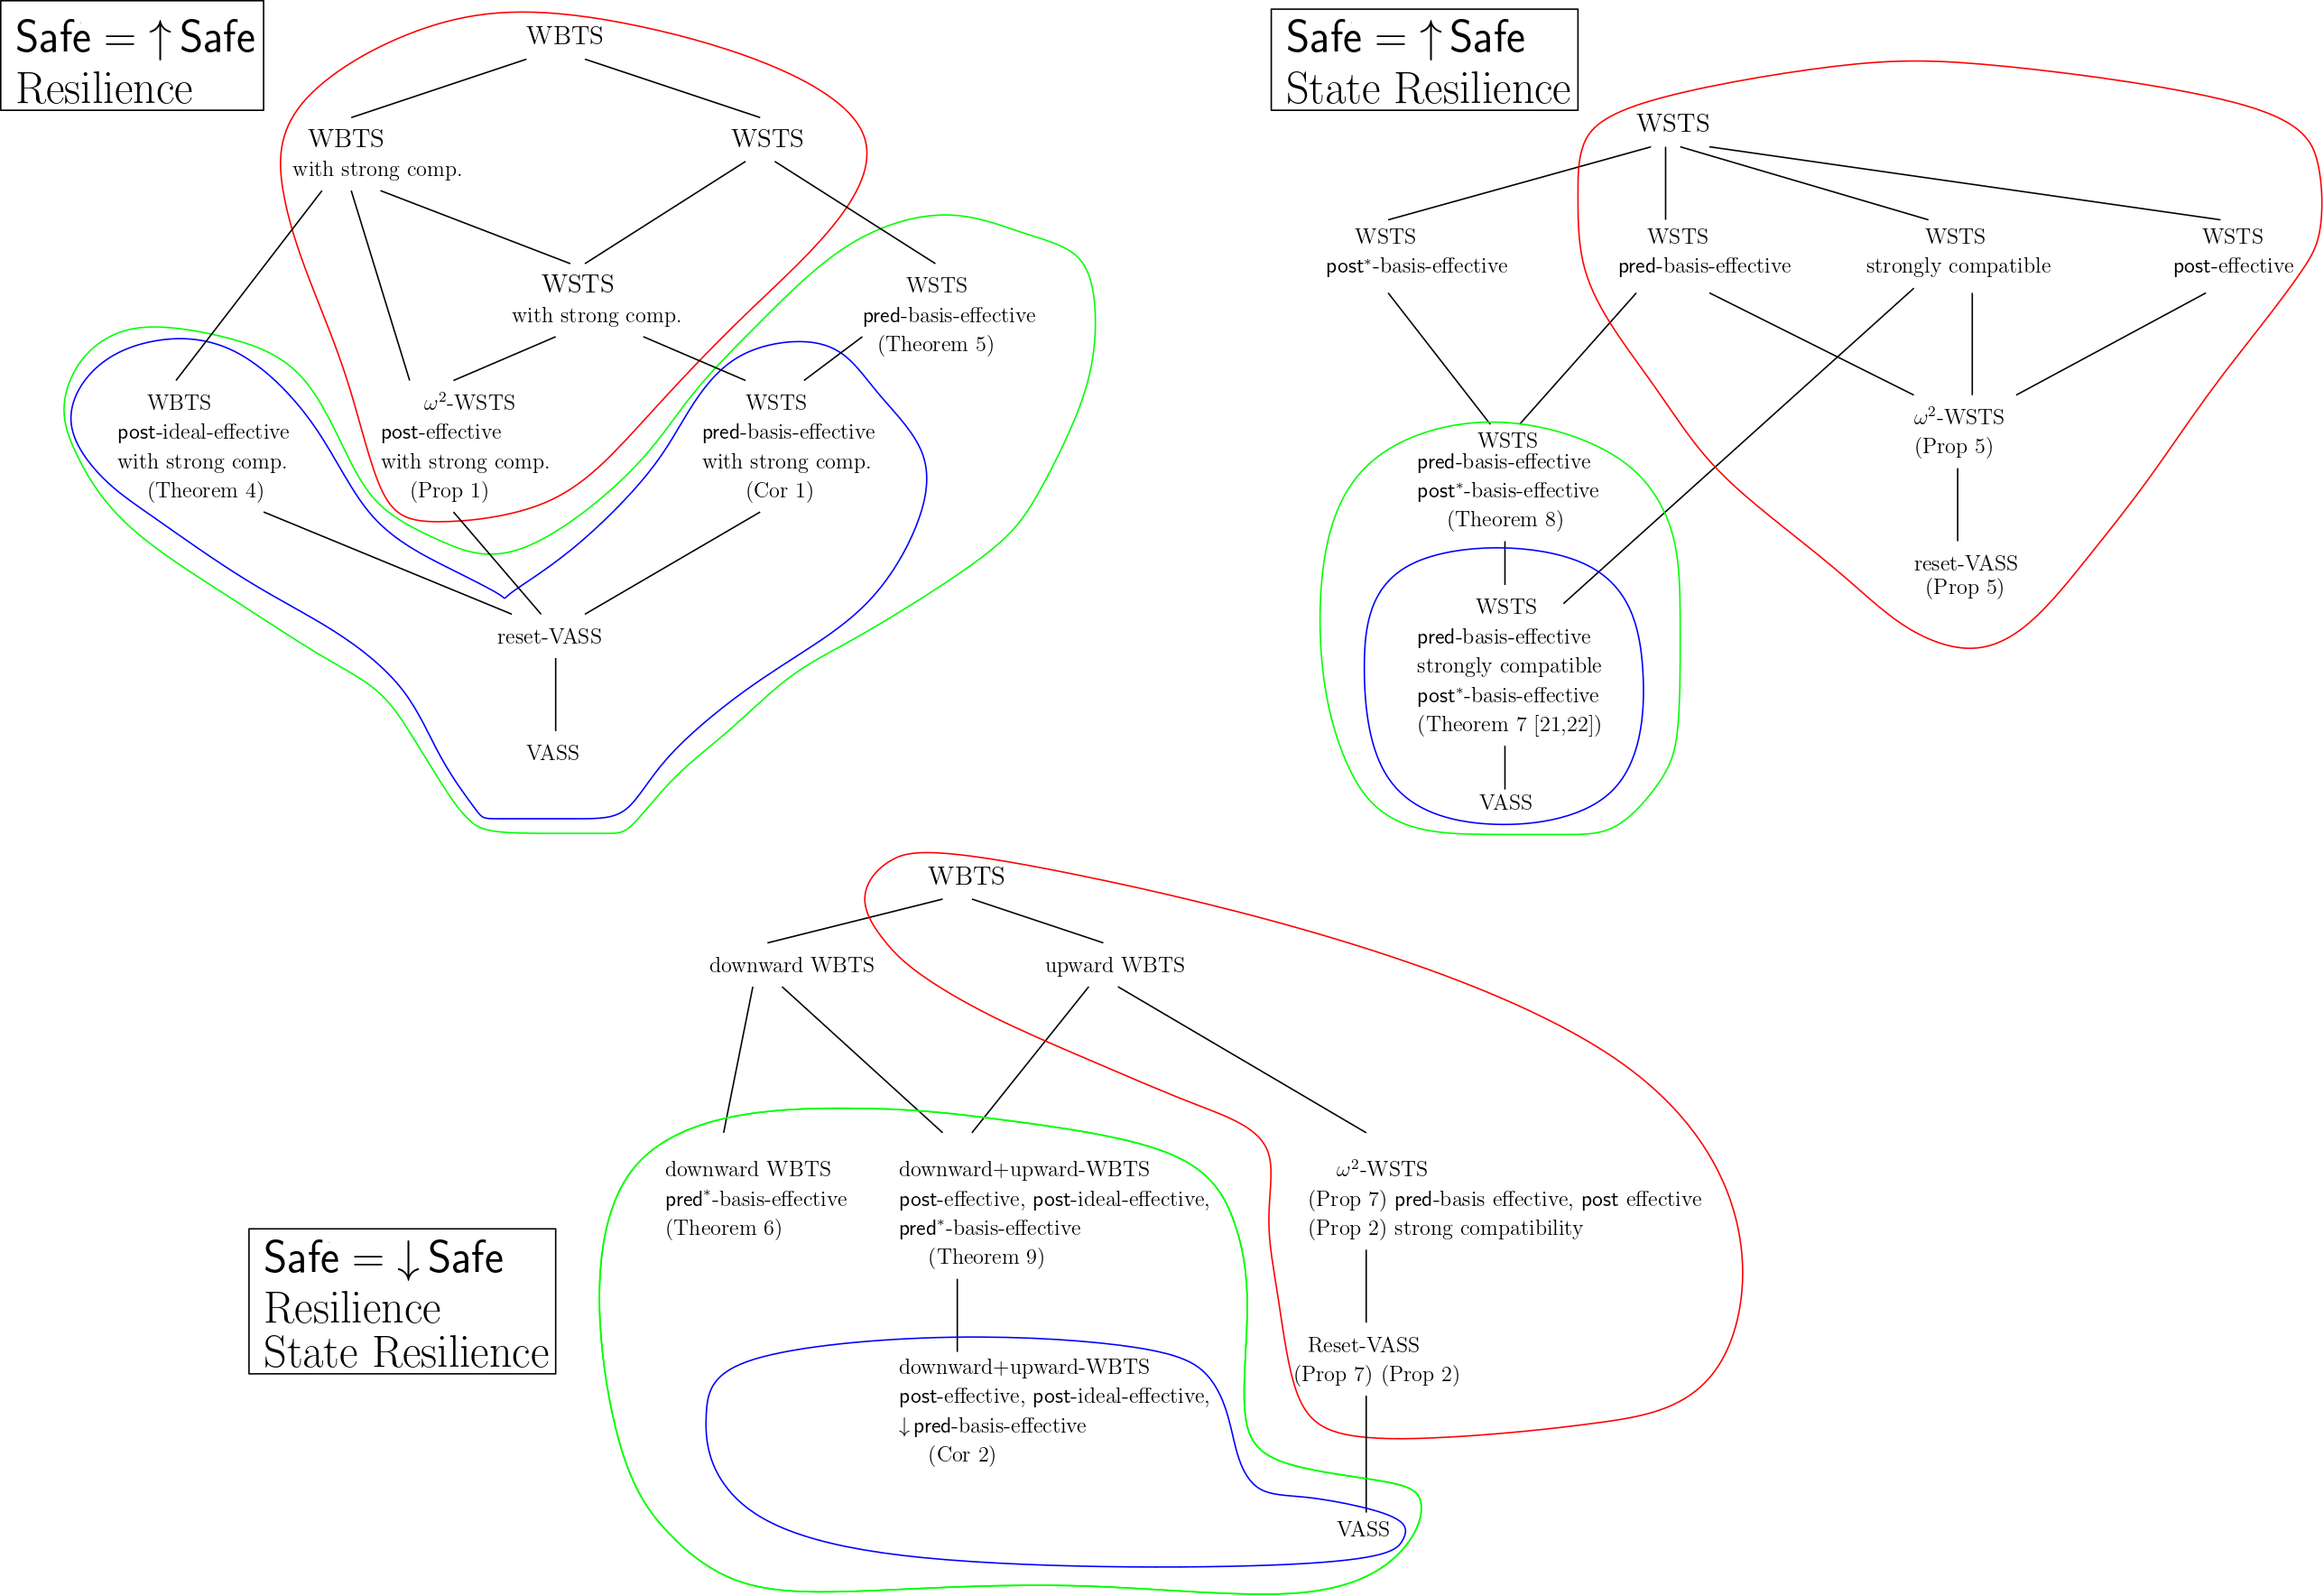
\includegraphics[width=1.00\textwidth]{All_results}
% \caption{Hasse diagram of some classes of transition systems, together with the decidability (in green) or undecidability (in red) of the resilience problems. Decidability of bounded resilience and $k-$resilience variants are indicated in blue.}
	\end{figure}
\end{center}  
    
    
        
  \end{frame}
%vvvvvvvvvvvvvvvvvvvvvvvvvvvvvvvvvvvvvvvvvvvvvvvvvvvvvvvvvvvvvvvvvvvvvvvvvv
  \begin{frame}{Results}
 
   \begin{center}
 	\begin{figure}
 	% \hspace{-2.cm}
 	\vspace{-0.25cm}
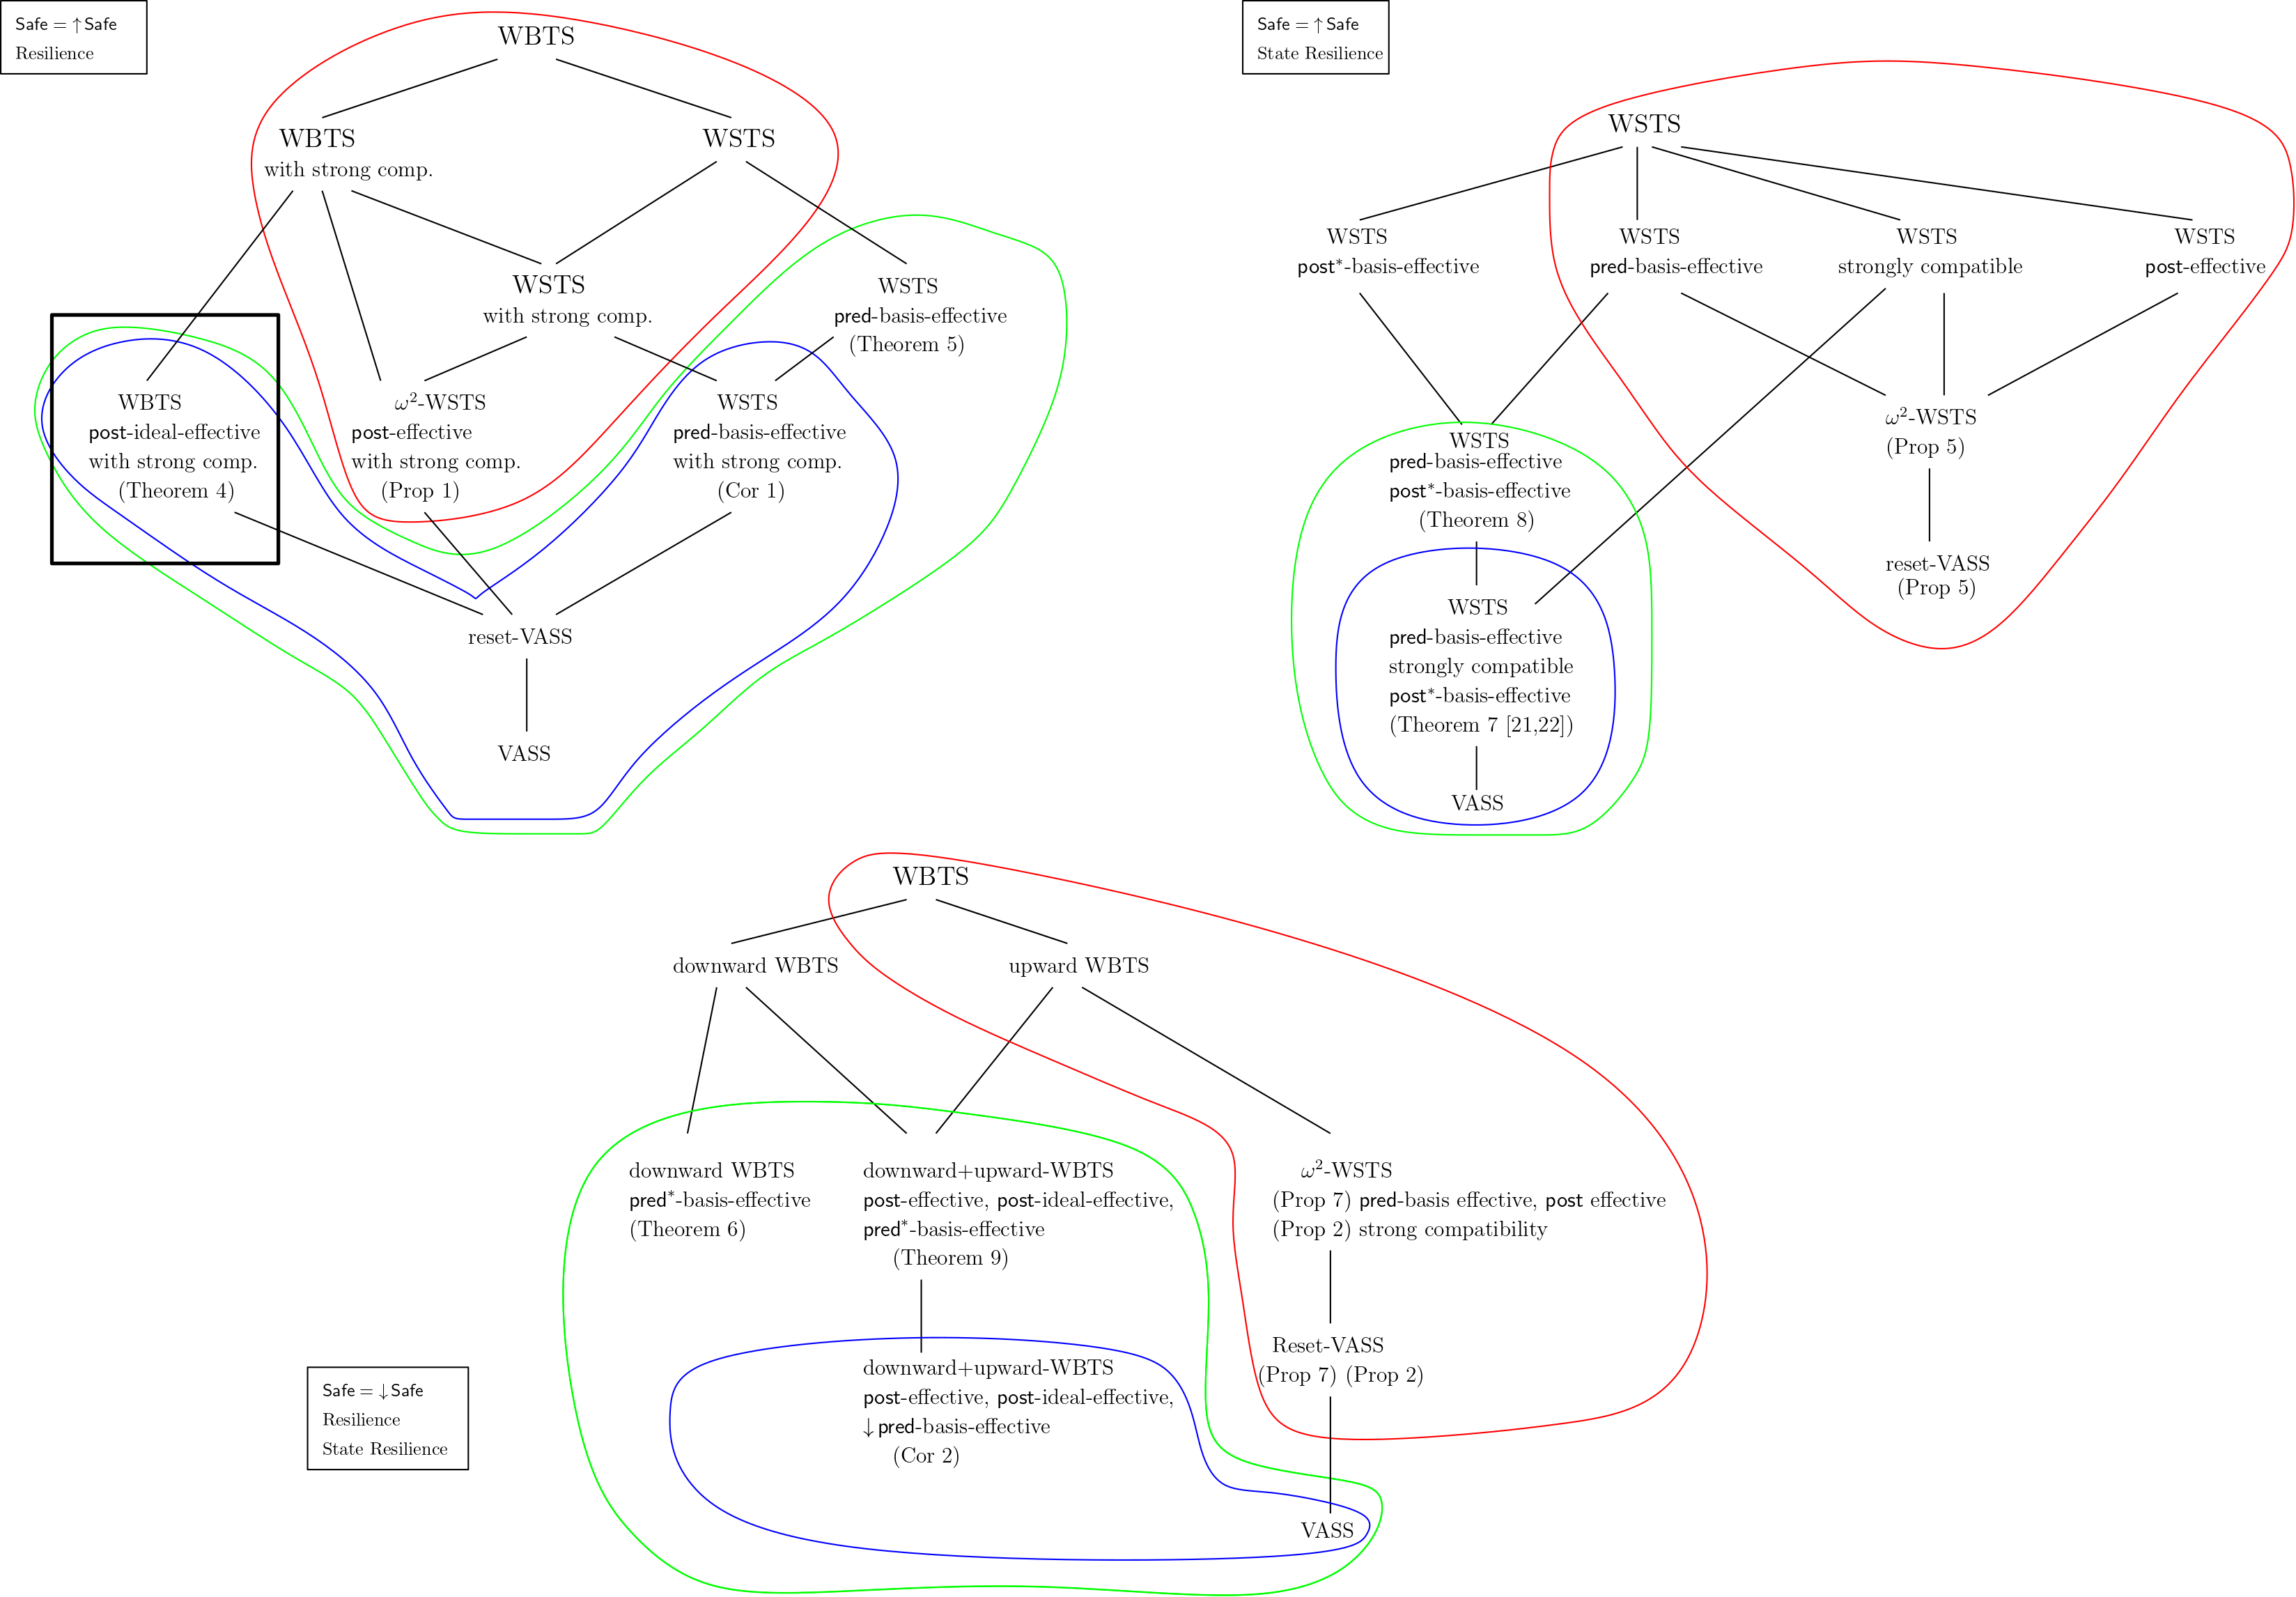
\includegraphics[width=1.00\textwidth]{resultA}
% \caption{Hasse diagram of some classes of transition systems, together with the decidability (in green) or undecidability (in red) of the resilience problems. Decidability of bounded resilience and $k-$resilience variants are indicated in blue.}
	\end{figure}
\end{center}  

  \end{frame}
%vvvvvvvvvvvvvvvvvvvvvvvvvvvvvvvvvvvvvvvvvvvvvvvvvvvvvvvvvvvvvvvvvvvvvvvvvv
  \begin{frame}{Ideals and effectivity}
  

$I$ Ideal =
\begin{itemize}
 \item Downward-closed % is any set $D \subseteq X$ such that if $y \leq x$ and $x \in D$ then $y \in D $. 
 ($y \leq x  \wedge x \in I \to y \in I$) 
 \item Directed % i.e. it is nonempty and for every $a,b \in D$, there exists $c \in D$ such that $a \leq c$ and $b \leq c$.
 ($I \neq \emptyset \wedge \forall a,b \in I, \exists c \in I, a \leq c \vee b \leq c$ )
\end{itemize} 

  
\hspace{-2cm}

$S$ effective = 
 \begin{itemize}
\item $s \to t$ decidable 
\item membership decidable 
\item $\leq$ decidable 
\item membership in $Ideals(S)$ decidable 
\item inclusion of ideals decidable
\end{itemize}



  \end{frame}
%vvvvvvvvvvvvvvvvvvvvvvvvvvvvvvvvvvvvvvvvvvvvvvvvvvvvvvvvvvvvvvvvvvvvvvvvvv
  \begin{frame}{Resilience when $\Safe = {\uparrow \Safe}$}
   
% Result A: Théorème 4 


% \begin{theorem}
% Let $\mathscr{S}=(S,\rightarrow, \leq)$ be a $\post$-ideal-effective WBTS with strong compatibility and a set $\Safe = \mathop{\uparrow} \Safe$.
% {\sc Resilience}, {\sc Bounded resilience} 
% and {\sc $k$-resilience} are decidable.
% \end{theorem}


\begin{block}{Theorem~4}
WBTS $\mathscr{S}=(S,\rightarrow, \leq)$ 
\begin{itemize}
\item effective + $\mathop{\downarrow} \post(I)$ computable$^1$ %$\post$-ideal-effective 
\item \textcolor{red}{strong} compatibility
\item $\Safe = \mathop{\uparrow} \Safe$
\end{itemize}
{\sc Resilience}, {\sc Bounded resilience} 
and {\sc $k$-resilience} decidable.
\end{block}


\begin{center}
 	\begin{figure}
 	% \hspace{-2.cm}
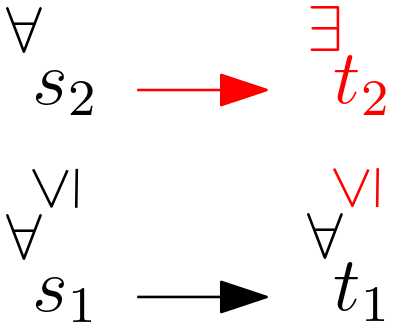
\includegraphics[width=.25\textwidth]{WSTS_strong}
	\end{figure}
\end{center}  

\phantom{Footnote}

{\small $^1$called $\post$-ideal-effective }

       \end{frame}
%vvvvvvvvvvvvvvvvvvvvvvvvvvvvvvvvvvvvvvvvvvvvvvvvvvvvvvvvvvvvvvvvvvvvvvvvvv
  \begin{frame}{Ingredient 1: link with coverability}
  

  \begin{block}{Reformulation}
Resilience $\equiv$ $\forall x \in \Bad$, $\exists y \in \Safe$, $y$ is coverable from $x$ ?
 \end{block}
 
 \pause

  \begin{block}{Proposition}
   $y$ is coverable from $x$ in $\mathscr{S}$ if and only if $\mathop{\downarrow} y$ is coverable from $\mathop{\downarrow} x$ in the completion $\hat{\mathscr{S}} $ 
 \end{block}
 
\pause

  \begin{block}{ }
This infinite set of coverability questions can be reduced to a \emph{finite} set of coverability questions in the completion $\hat{\mathscr{S}}=(Ideals(S),\rightarrow, \subseteq)$ of $\mathscr{S}=(S,\rightarrow, \leq)$. 
 \end{block}
 


  \end{frame}
%vvvvvvvvvvvvvvvvvvvvvvvvvvvvvvvvvvvvvvvvvvvvvvvvvvvvvvvvvvvvvvvvvvvvvvvvvv
  \begin{frame}{Ingredient 2: the completion}
 
 
 \begin{definition}[\cite{BFM-ic17}]
The \emph{completion}   of a WBTS $\mathscr{S}=(S,\rightarrow, \leq)$ is the associated ordered transition system $\hat{\mathscr{S}}=(Ideals(S),\rightarrow, \subseteq)$ where 
%$Ideals(S)$ is the set of ideals of $S$ and
 $I \rightarrow J$ if $J$ belongs to the finite ideal decomposition of $\mathop{\downarrow} \post_{\mathscr{S}}(I)$. 
% The completion is always \emph{finitely branching} but it is not necessarly a WSTS since $\subseteq$ is not necessarly a wqo. 
%It is proved in  \cite{BFM-ic17} that $\hat{\mathscr{S}}$ is WSTS iff $\mathscr{S}=(S,\rightarrow, \leq)$ is $\omega^2$-WSTS. \\
\end{definition}



\pause

\begin{exampleblock}{From a WBTS to its completion}
If $x \xrightarrow{k} y$ in $\mathscr{S}$ then for every ideal $I \supseteq \mathop{\downarrow} x$, there exists an ideal $J \supseteq \mathop{\downarrow} y$ such that $I \xrightarrow{k} J$ in $\hat{\mathscr{S}}$.
\end{exampleblock}


\pause

\begin{exampleblock}{From the completion to the WBTS}
If $I \xrightarrow{k} J$ in $\hat{\mathscr{S}}$ then for every $y \in J$, there exists $x \in I$ and $y' \geq y$ such that $x \xrightarrow{k'} y'$ in $\mathscr{S}$. If $\mathscr{S}$ has strong compatibility then $k’ = k$.
\end{exampleblock}



 
  

  \end{frame}
  %vvvvvvvvvvvvvvvvvvvvvvvvvvvvvvvvvvvvvvvvvvvvvvvvvvvvvvvvvvvvvvvvvvvvvvvvvv
    \begin{frame}{Results}
  
% Now that everything is somewhat properly defined maybe the picture with all the results ?  
  
   \begin{center}
 	\begin{figure}
 	% \hspace{-2.cm}
 	\vspace{-0.25cm}
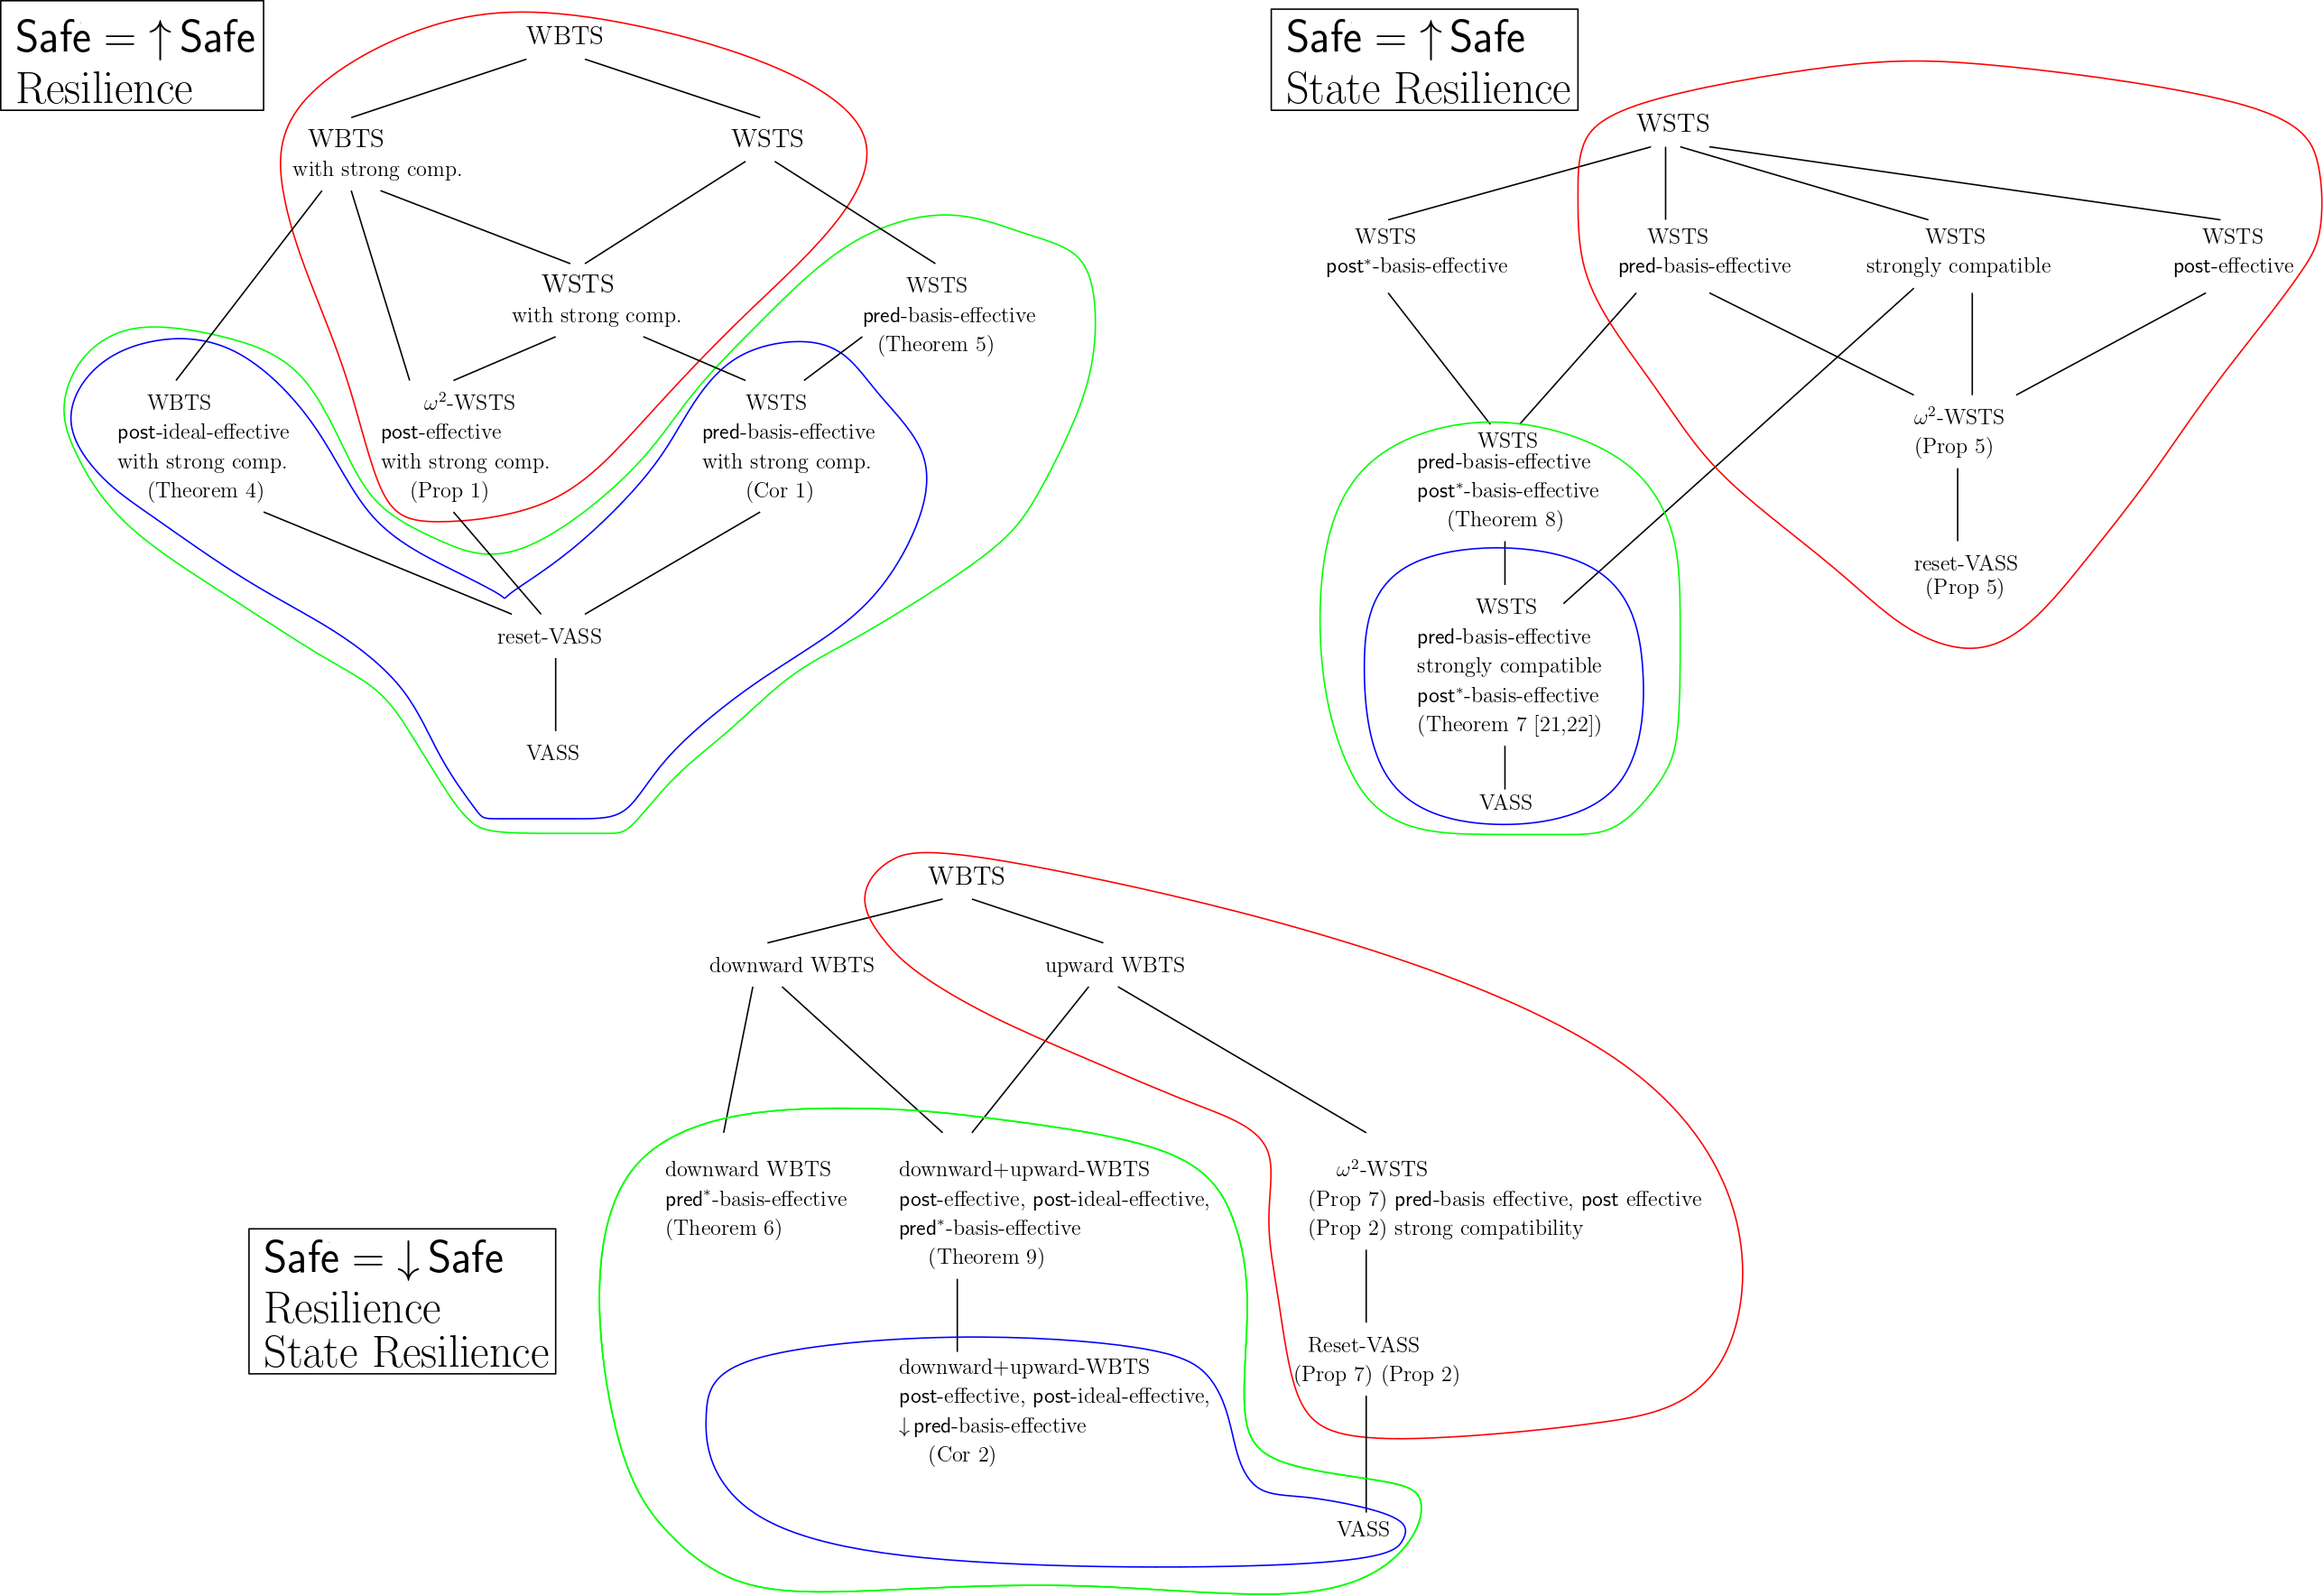
\includegraphics[width=1.00\textwidth]{All_results}
% \caption{Hasse diagram of some classes of transition systems, together with the decidability (in green) or undecidability (in red) of the resilience problems. Decidability of bounded resilience and $k-$resilience variants are indicated in blue.}
	\end{figure}
\end{center}  
    
    
          \end{frame}
%vvvvvvvvvvvvvvvvvvvvvvvvvvvvvvvvvvvvvvvvvvvvvvvvvvvvvvvvvvvvvvvvvvvvvvvvvv
  \begin{frame}{State resilience}
 
   \begin{center}
 	\begin{figure}
 	% \hspace{-2.cm}
 	\vspace{-0.25cm}
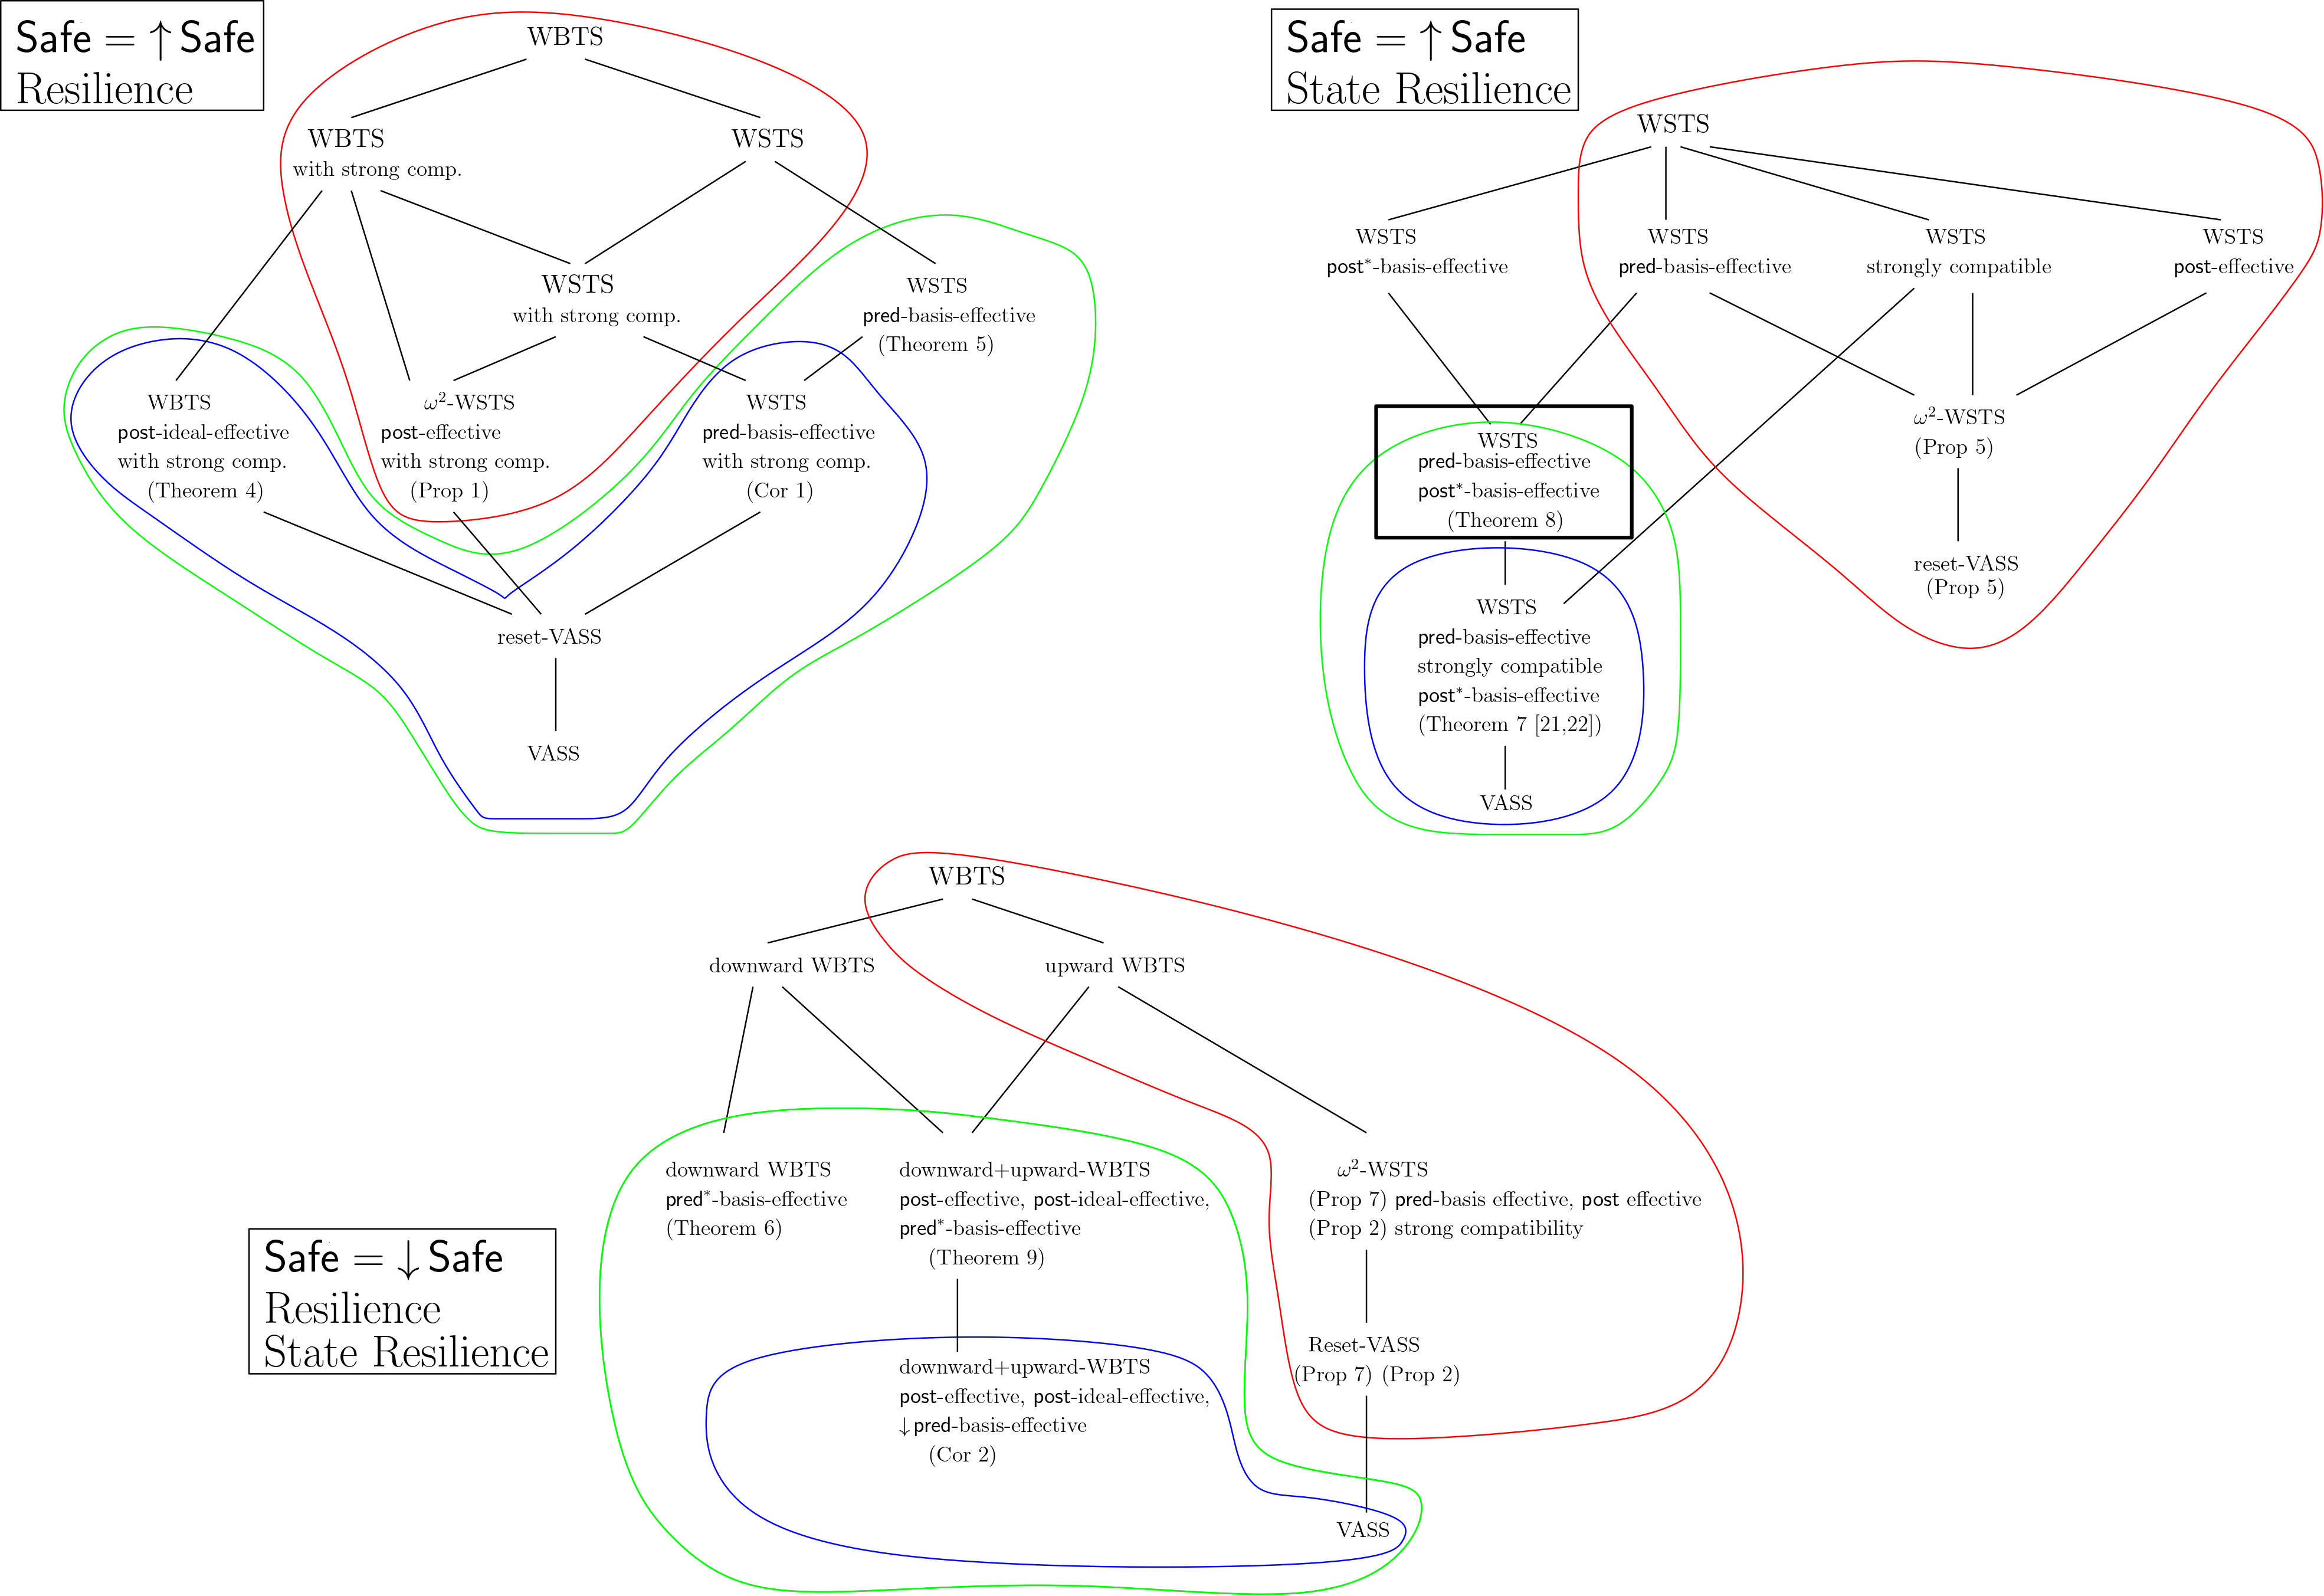
\includegraphics[width=1.00\textwidth]{resultB}
% \caption{Hasse diagram of some classes of transition systems, together with the decidability (in green) or undecidability (in red) of the resilience problems. Decidability of bounded resilience and $k-$resilience variants are indicated in blue.}
	\end{figure}
\end{center}  



\nocite{DBLP:conf/gg/Ozkan22}
 
  \end{frame}
%vvvvvvvvvvvvvvvvvvvvvvvvvvvvvvvvvvvvvvvvvvvvvvvvvvvvvvvvvvvvvvvvvvvvvvvvvv
  \begin{frame}{Resilience $\ldots$}
  
% Now that everything is somewhat properly defined maybe the picture with all the results ?  
  
   \begin{center}
 	\begin{figure}
 	% \hspace{-2.cm}
 	\vspace{-0.25cm}
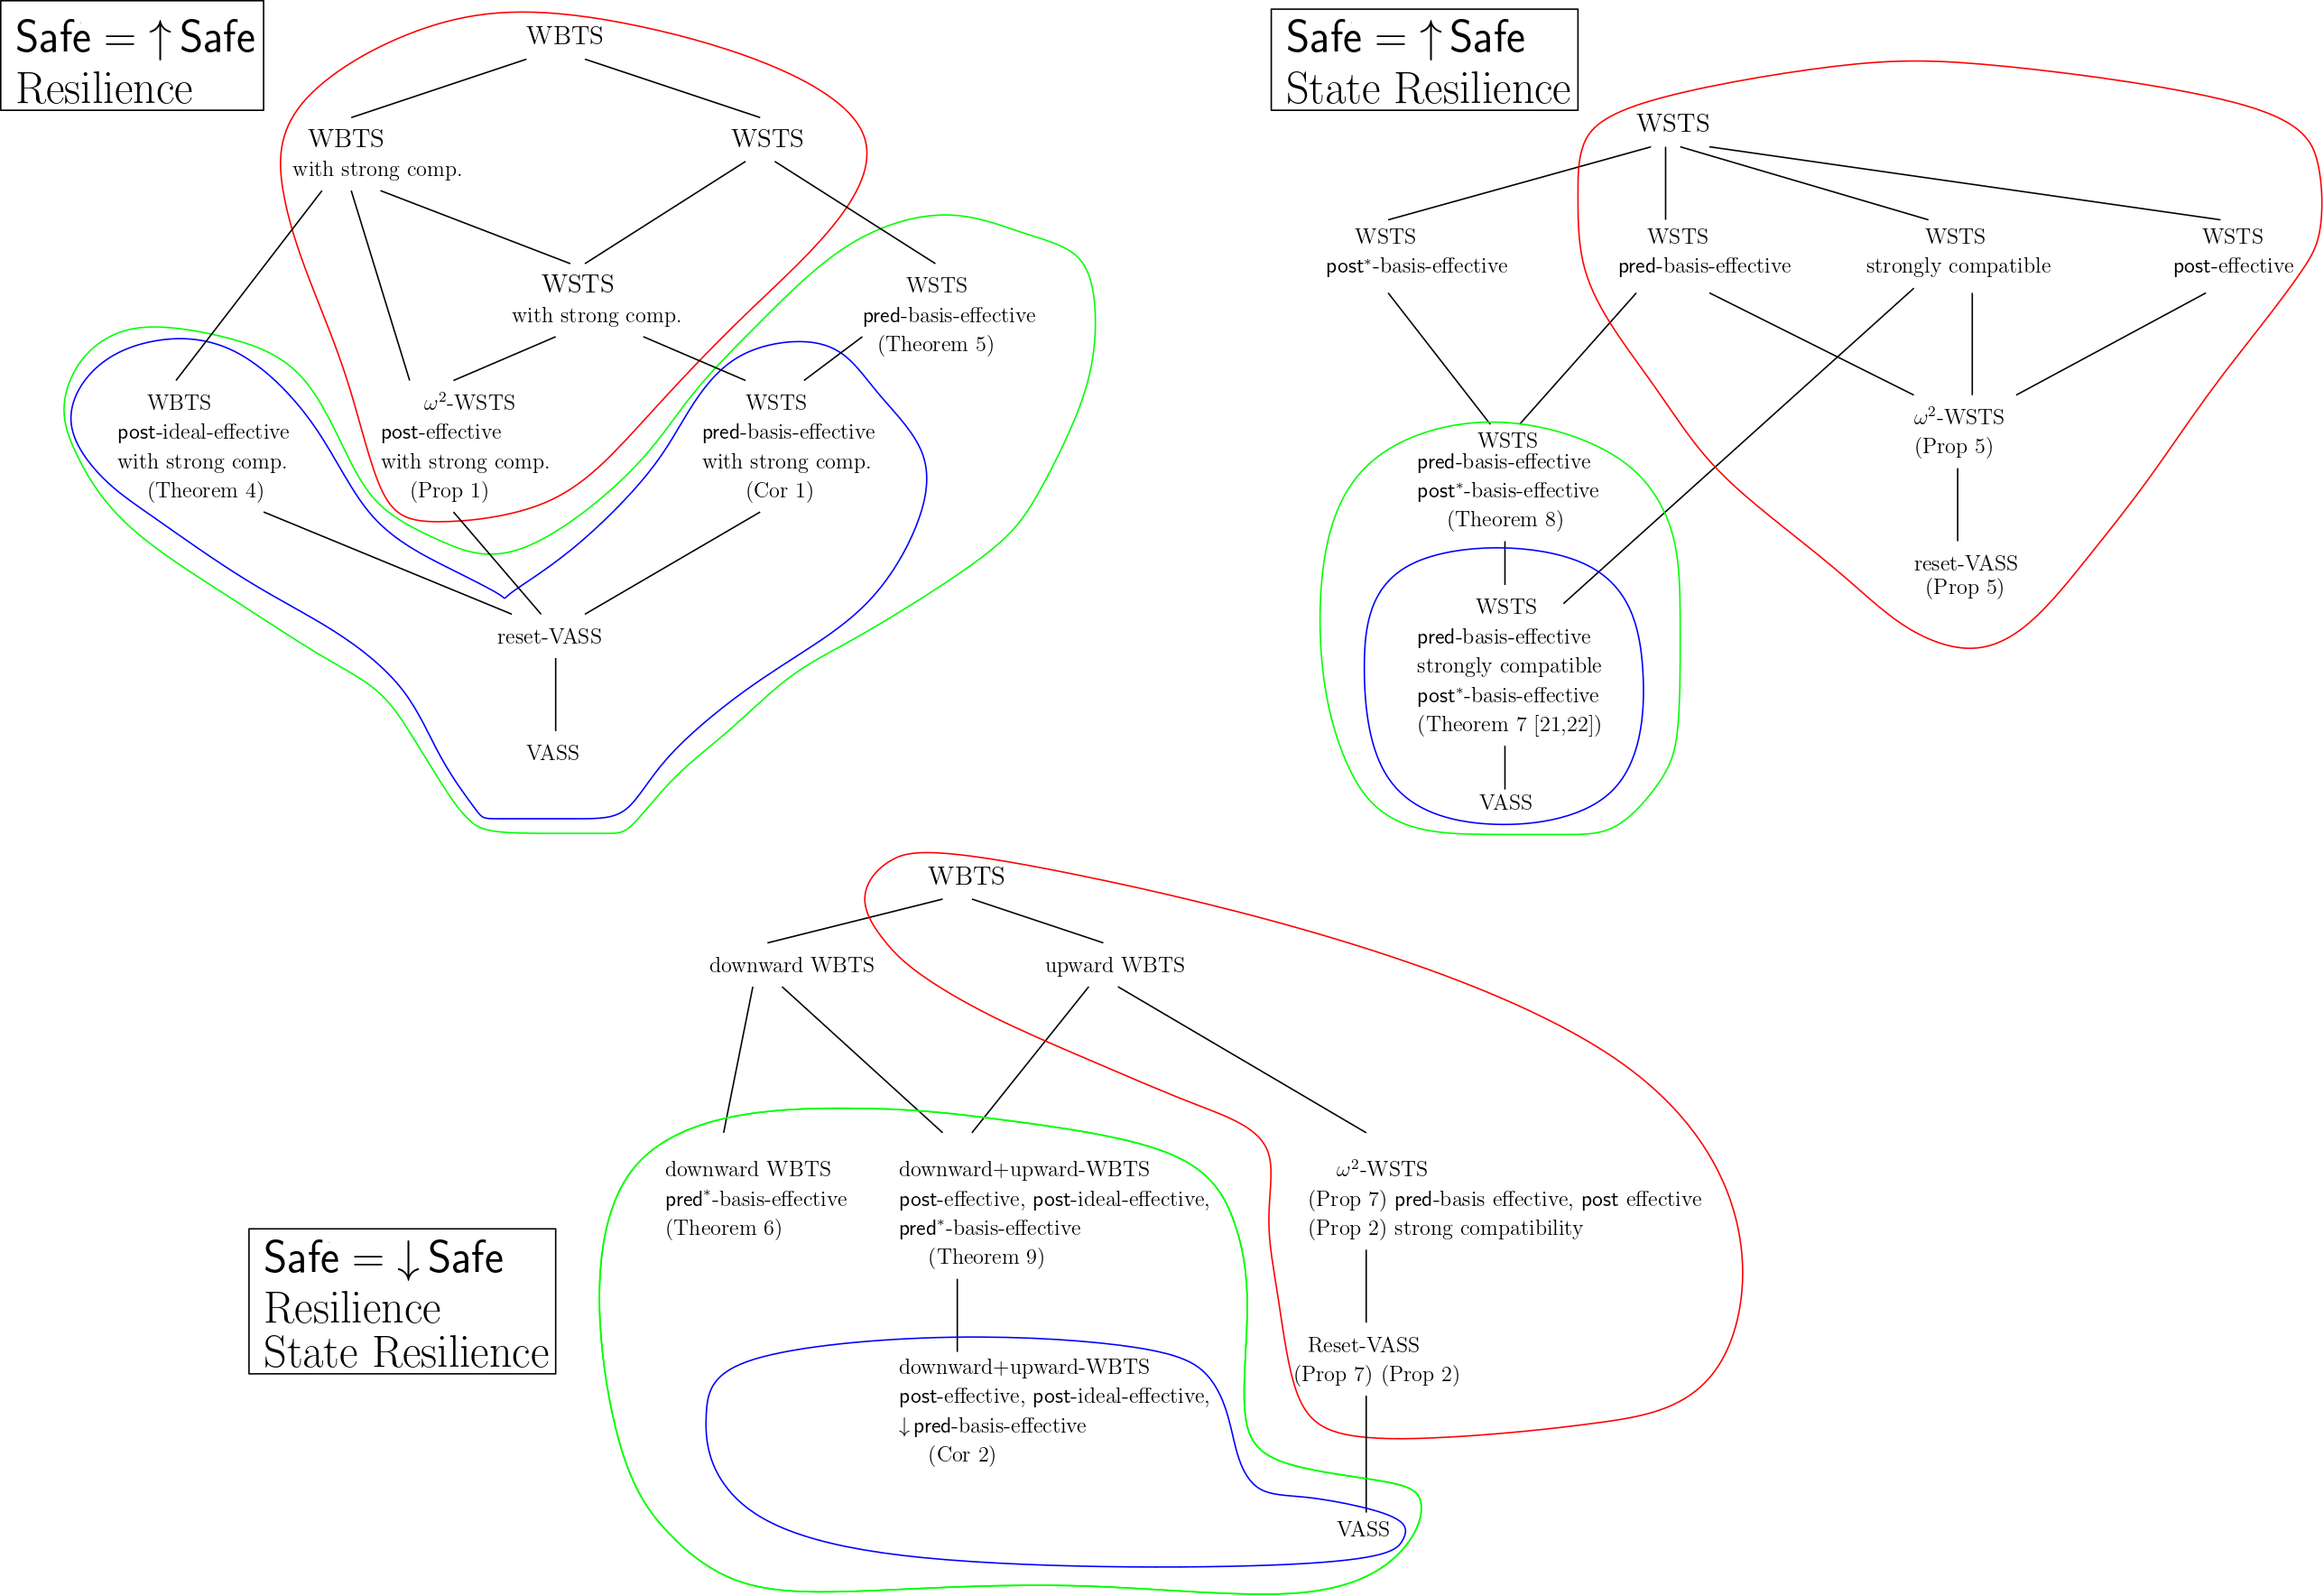
\includegraphics[width=1.00\textwidth]{All_results}
% \caption{Hasse diagram of some classes of transition systems, together with the decidability (in green) or undecidability (in red) of the resilience problems. Decidability of bounded resilience and $k-$resilience variants are indicated in blue.}
	\end{figure}
\end{center}  
    
    

  \end{frame}
%vvvvvvvvvvvvvvvvvvvvvvvvvvvvvvvvvvvvvvvvvvvvvvvvvvvvvvvvvvvvvvvvvvvvvvvvvv
  \begin{frame}{Resilience $\ldots$ for VASS}
 
   \begin{center}
 	\begin{figure}
 	% \hspace{-2.cm}
 	\vspace{-0.25cm}
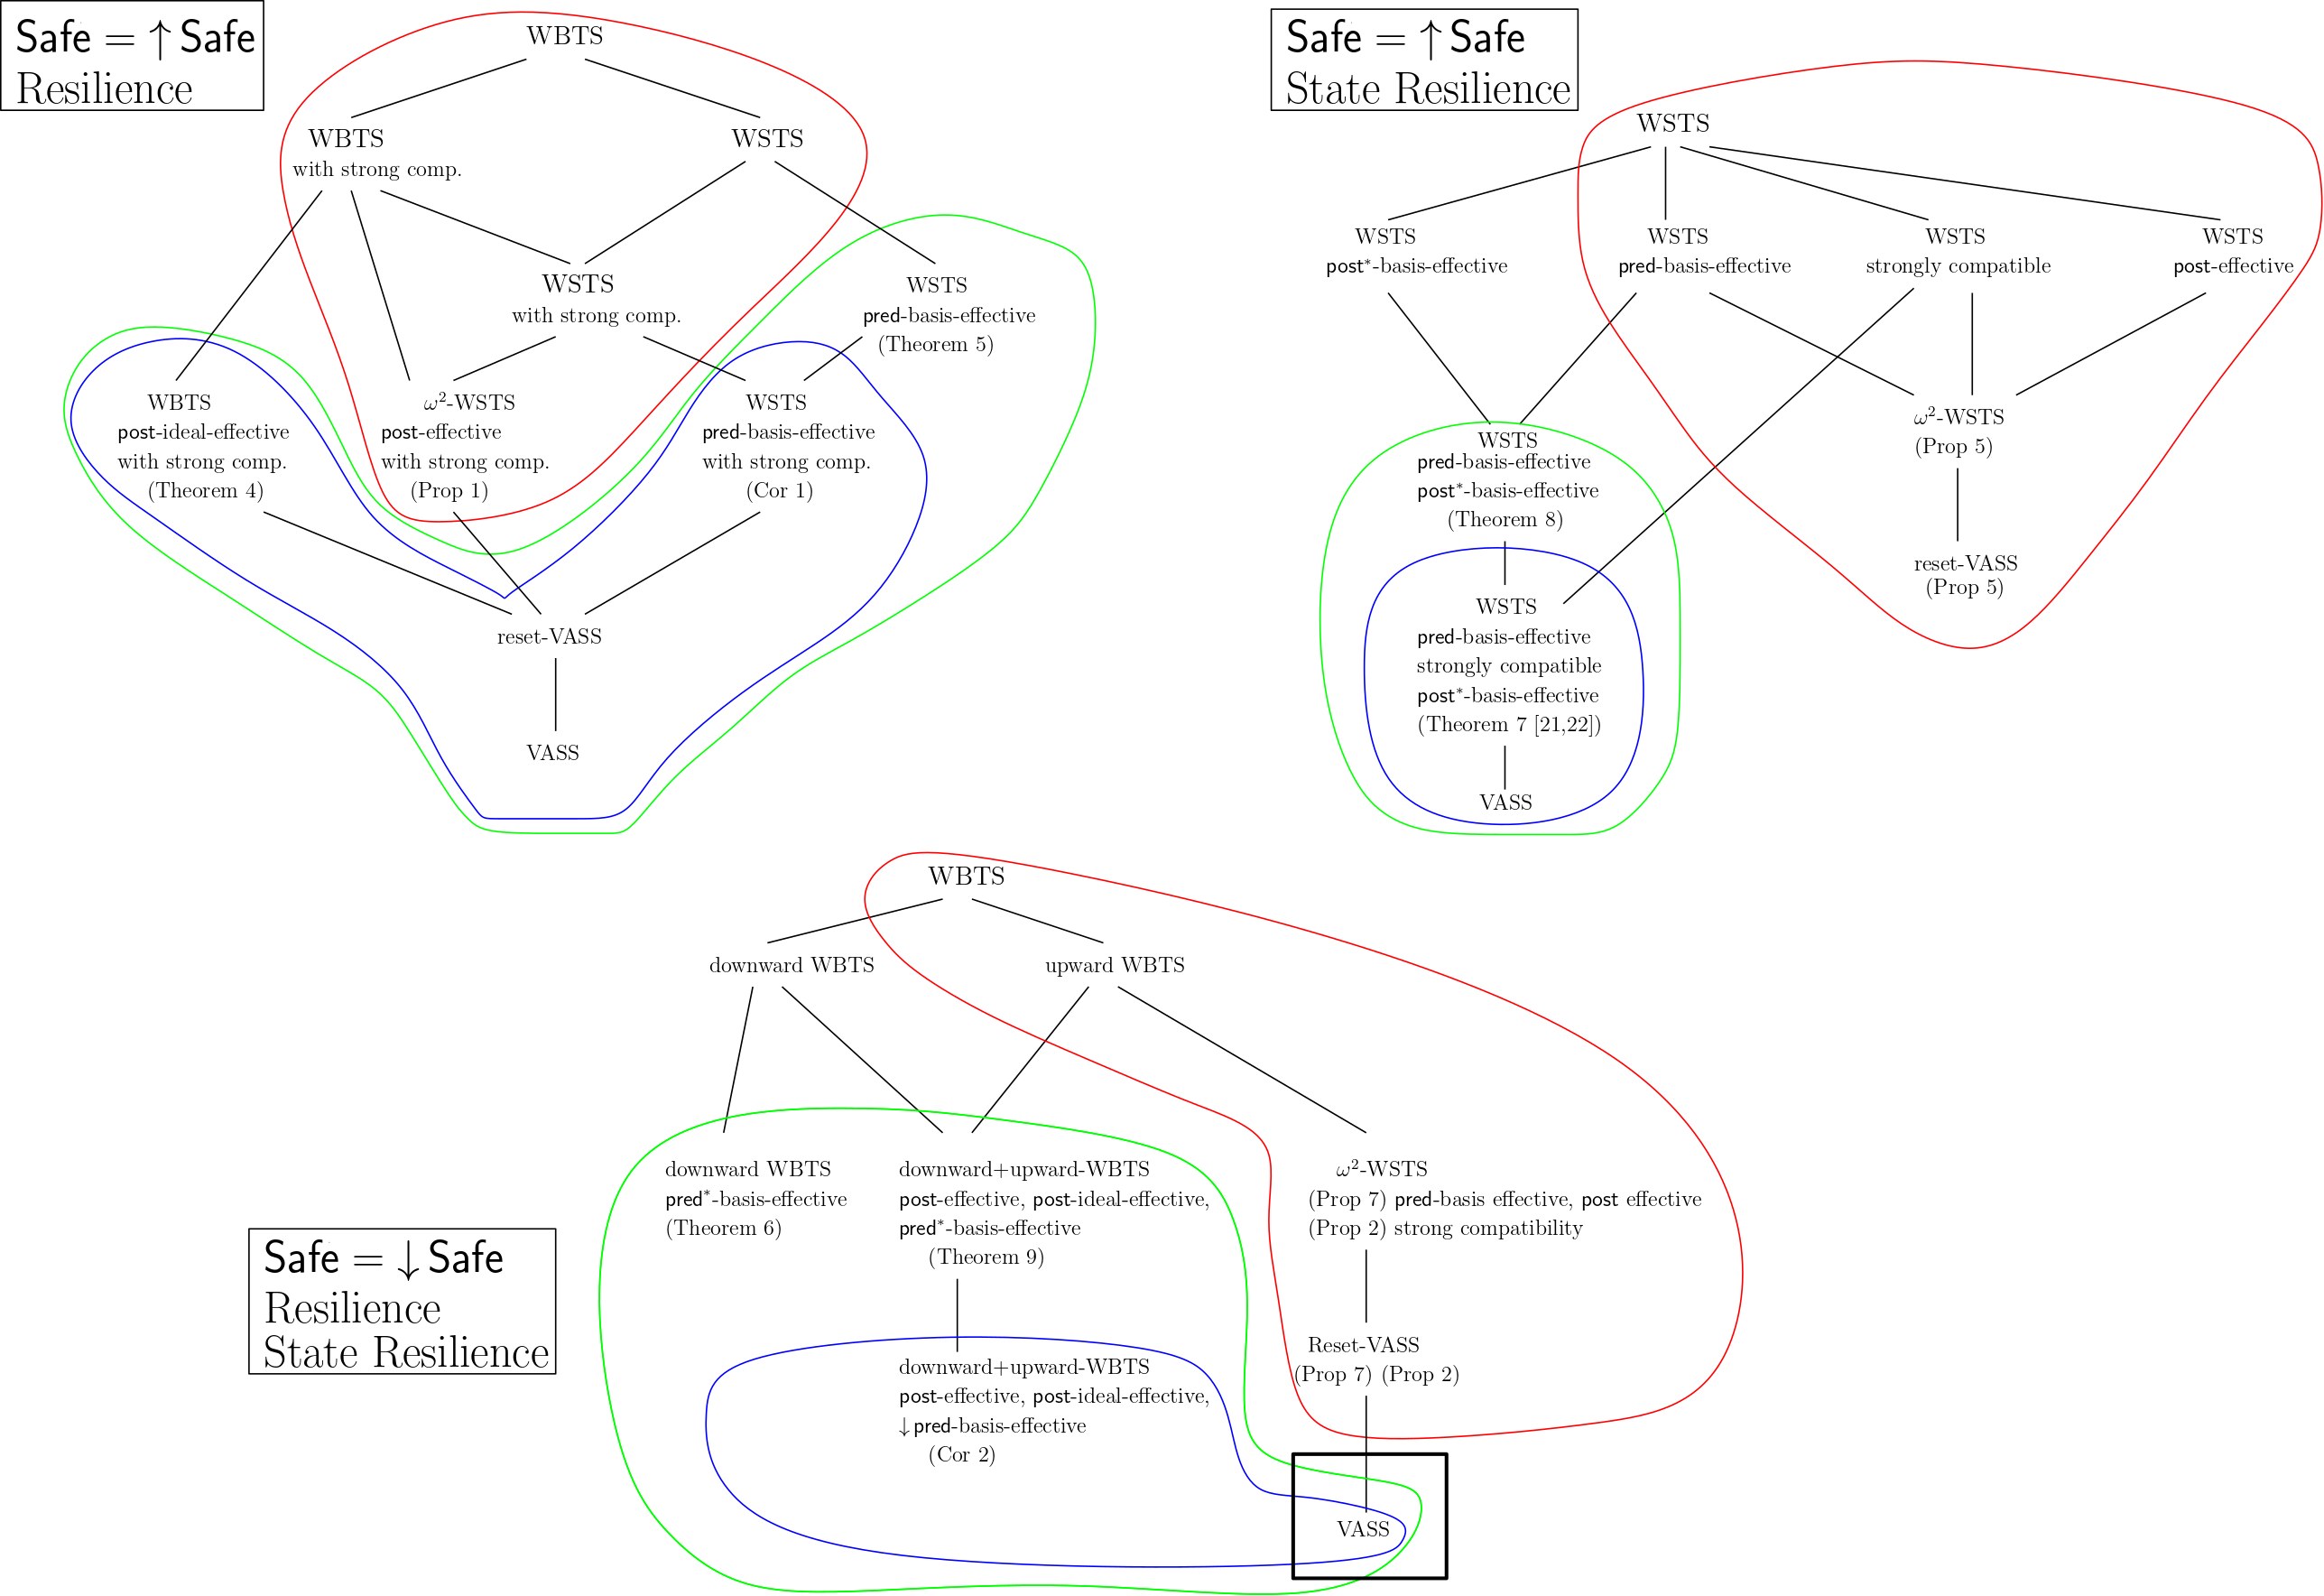
\includegraphics[width=1.00\textwidth]{resultC}
% \caption{Hasse diagram of some classes of transition systems, together with the decidability (in green) or undecidability (in red) of the resilience problems. Decidability of bounded resilience and $k-$resilience variants are indicated in blue.}
	\end{figure}
\end{center}  


  \end{frame}
%vvvvvvvvvvvvvvvvvvvvvvvvvvvvvvvvvvvvvvvvvvvvvvvvvvvvvvvvvvvvvvvvvvvvvvvvvv
  \begin{frame}{Vector Addition System with States}
  
   \begin{center}
 	\begin{figure}
 	\vspace{.06cm}
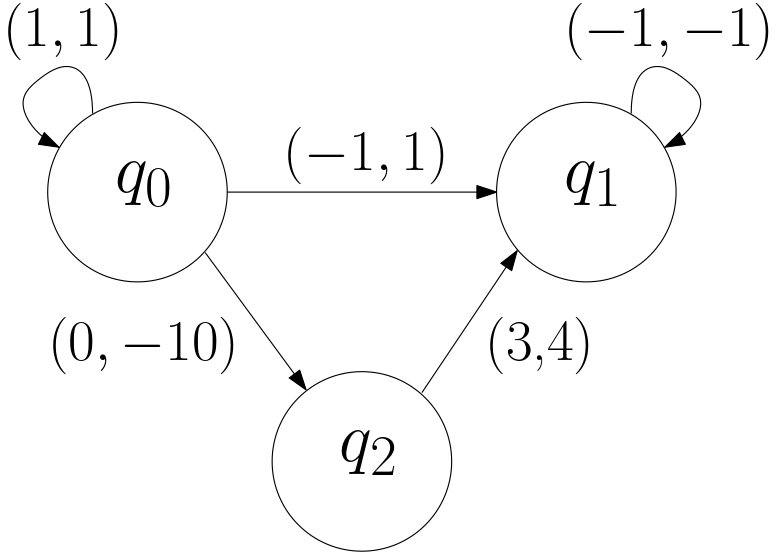
\includegraphics[width=.4\textwidth]{FigC}
	\end{figure}
\end{center}  

  \end{frame}
%vvvvvvvvvvvvvvvvvvvvvvvvvvvvvvvvvvvvvvvvvvvvvvvvvvvvvvvvvvvvvvvvvvvvvvvvvv
  \begin{frame}{Resilience(s) for VASS and VAS}

\begin{block}{Theorem}
{\sc Resilience} is decidable for VASS, and $\mathbb{Z}-$VASS, when $\Safe$  is a semilinear set.
\end{block}


$\to$ it is decidable whether $\post^*(\Bad) \subseteq \pred^*(\Safe)$ when 
$\Bad$ and $\Safe$ are both semilinear~\cite{DBLP:journals/corr/abs-2207-02697}

\pause 

\begin{block}{Theorem}
{\sc Bounded resilience} and {\sc $k$-resilience } are decidable for VASS when 
$\Safe = \mathop{\downarrow} \Safe$.
\end{block}

 
\pause

\begin{block}{Proposition}
{\sc Bounded resilience} and {\sc $k$-resilience} never hold for $d$-VAS when $\Safe = \mathop{\downarrow} \Safe \neq \N^d$.
\end{block}





  \end{frame}
%vvvvvvvvvvvvvvvvvvvvvvvvvvvvvvvvvvvvvvvvvvvvvvvvvvvvvvvvvvvvvvvvvvvvvvvvvv
  \begin{frame}{Conclusion}
  
   \begin{center}
 	\begin{figure}
 	% \hspace{-2.cm}
 	\vspace{-0.25cm}
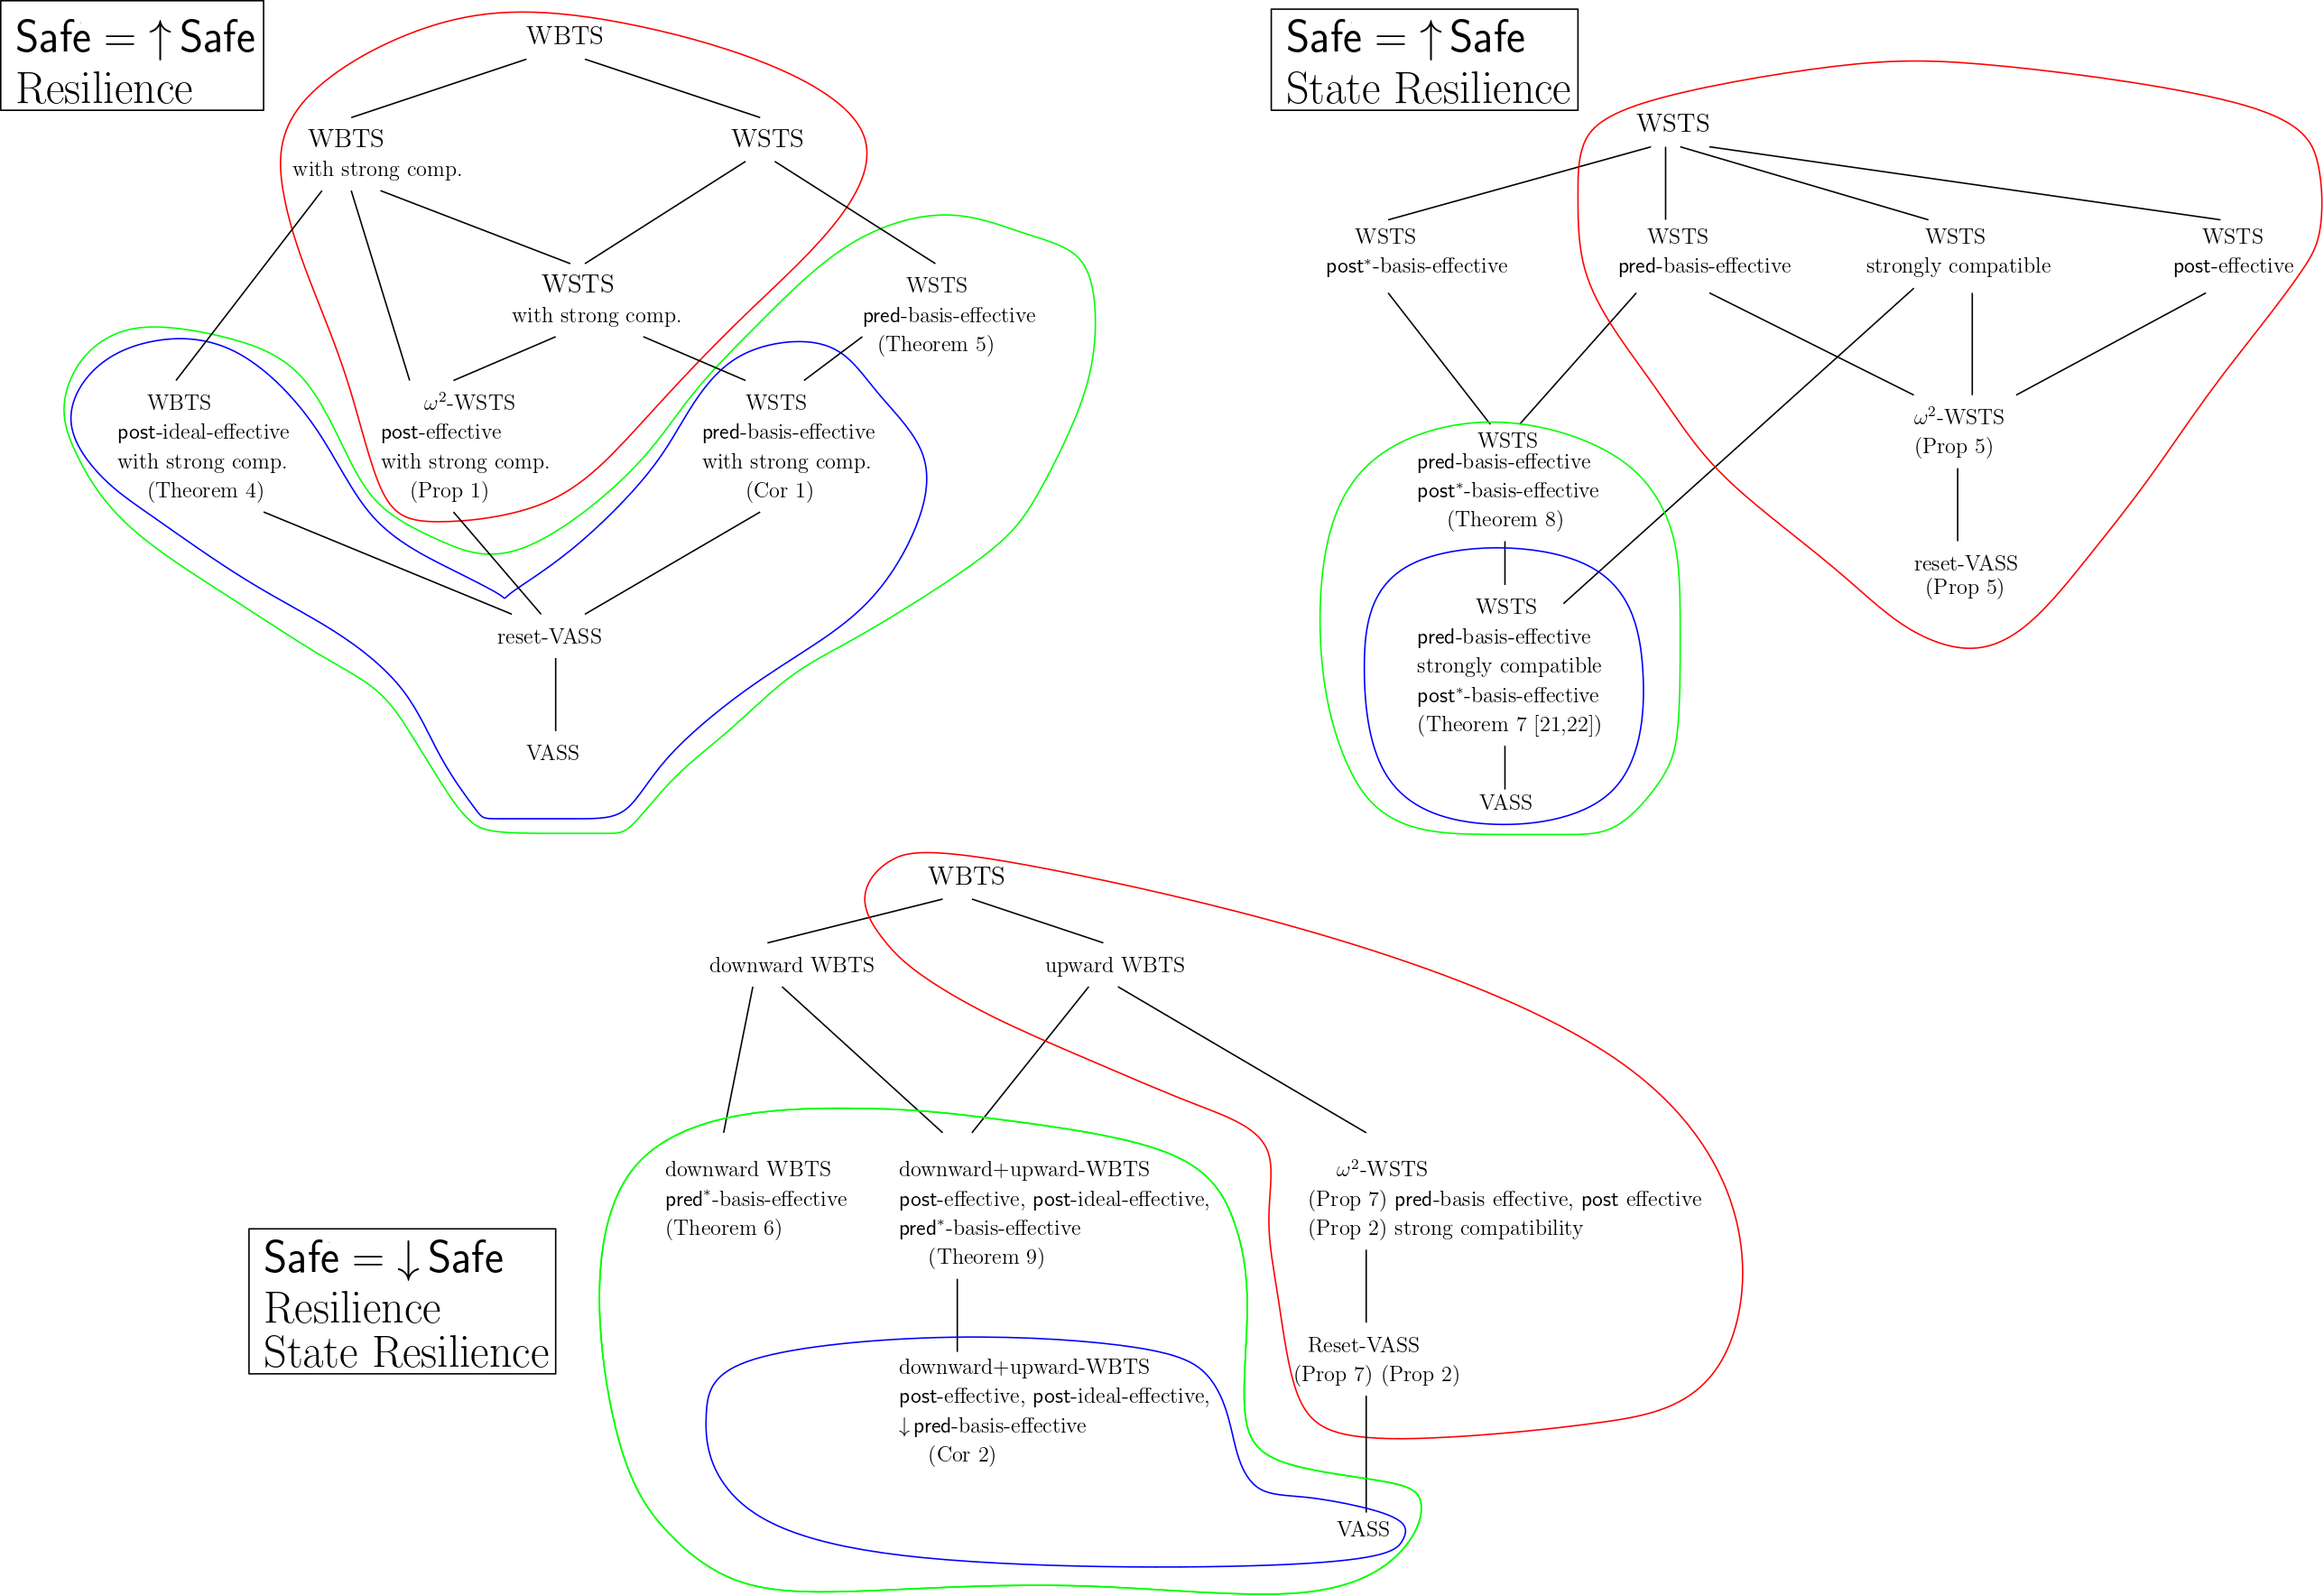
\includegraphics[width=1.00\textwidth]{All_results}
% \caption{Hasse diagram of some classes of transition systems, together with the decidability (in green) or undecidability (in red) of the resilience problems. Decidability of bounded resilience and $k-$resilience variants are indicated in blue.}
	\end{figure}
\end{center}  
    
% How to expand current results ?

% - detailed complexity analysis (in VASS \& variations)

% - other classes of $\Safe / \Bad$ (e.g. semilinear)

  \end{frame}
%vvvvvvvvvvvvvvvvvvvvvvvvvvvvvvvvvvvvvvvvvvvvvvvvvvvvvvvvvvvvvvvvvvvvvvvvvv
  \begin{frame}{References}
      
      {\tiny
\bibliography{bib}
}

  \end{frame}
%vvvvvvvvvvvvvvvvvvvvvvvvvvvvvvvvvvvvvvvvvvvvvvvvvvvvvvvvvvvvvvvvvvvvvvvvvv
  \begin{frame}
  
  \begin{center}
  Thanks for your attention
  \end{center}
  


  \end{frame}
%vvvvvvvvvvvvvvvvvvvvvvvvvvvvvvvvvvvvvvvvvvvvvvvvvvvvvvvvvvvvvvvvvvvvvvvvvv

 
  
\end{document}
